\cleardoublepage


\chapter{Image/Video Feature Extraction }
\label{ch:computervision}

\par The task of automatically recognizing and locating objects in images and videos is of extreme importance for computers to be able to understand and interact with their surroundings. Some major applications of this particular task are pedestrian face detection, surveillance, autonomous driving and text digitalization, where object detection is a crucial challenge. \cite{Agarwal2019}


\par Feature extraction plays an important role in image classification and object detection systems which are two core components of computer vision. It is characterized by two important aspects, the mapping of image pixels into the feature space (explained in more details in section \ref{sec:featurespace}) and with the extraction of various attributes of an object. Only after extracting useful features from either images or videos, the computer is able to define what an object is or what a certain environment contains.\cite{Tiwari2013}

Putting it simply, feature extraction is the first step to convert an image into text.

\begin{figure}[htb]
    \centering
    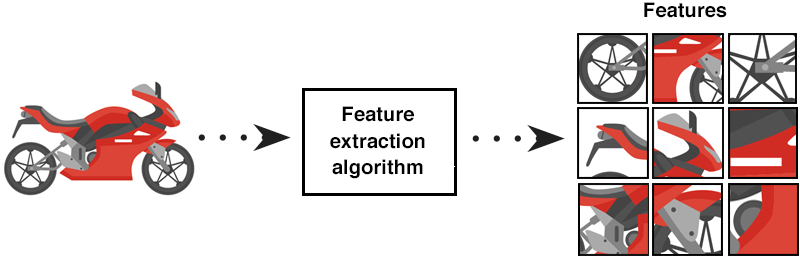
\includegraphics[scale = 0.55]{Sections/2StateOfTheArt/2_images/Feature_extraction.png}
    \caption{Feature extraction from an image. \cite{feature} }  
\end{figure}


\par This chapter starts with fundamental concepts in order to understand how feature extraction in computer vision works. Section \ref{sec:libraries} gives a brief introduction of the most common computer vision libraries. Neural networks are introduced in section \ref{sec:neuralnet}, where the most common architecture types are presented. All CNN architectures and regression based algorithms used during the development of this thesis are explained with detail in sections \ref{sec:cnn} and \ref{sec:regression}. Classification based algorithms, presented in \ref{sec:classification}, were not used in this work, but they are a required reading in order to understand the differences between them and the regression based algorithms. Finally, a state-of-the-art in object detection and image classification can be read in section \ref{sec:state}.

\newpage

%%%%%%%%%%%%%%%%%%%%%%%%%%%%%%%%%%%%%%%%%%%%%%%%%%%%%%%%%%%%%%%%%%%%%%%%%%%%%%

\section{Fundamental Concepts}
%%%%%%%%%%%%%%%%%%%%%%%%%%%%%%%%%%%%%%%%%%%%%%%%%%%%%%%%%%%%%%%%%%%%%%%%%%%%%%
    \subsection{Artificial Intelligence}
    \par Artificial Intelligence (AI) is the artificial simulation of human intelligence by a computer system in a way that it can perceive its environment, understand its behaviors and take action. Two important areas of AI are machine learning and deep learning. \cite{mathworks_AI}

    \subsection{Machine Learning}



    \par Machine learning can be defined as a data analytics technique that allows computers to learn from experience. There are two types of machine learning techniques, which are supervised learning and unsupervised learning.
    \par Normally, supervised machine learning is used to train a model to predict future outputs, this is done by inputting and outputting known data. Supervised learning uses two different techniques which are classification and regression. Classification techniques are used to classify input data into categories while regression techniques are used to predict continuous responses. 
    \par Unsupervised learning is mostly used to find hidden patterns or intrinsic structures in input data. The most common unsupervised learning technique is clustering which is used for data analysis exploration, in order to find hidden patterns or groupings in data. \cite{mathworks_NN}

    \subsection{Deep Learning}


    \par Deep Learning is a subset of Machine Learning that is inspired by the structure and function of the human brain. In order to achieve this, deep learning resorts to artificial neural networks (ANNs).
    
    \par The idea behind an ANN is that it tries to replicate the working of the human brain in the processing of data and creation of patterns, which is important for decision making. These ANNs are capable of learning unsupervised data that can either be unstructured, unlabeled or both. 
    
    \par Putting it as simple as possible, deep learning is a machine learning technique that teaches computers to learn by example, like a human would. \cite{mathworks_deeplearning}


    \par Thanks to the new digital era, there has been an exponential increase in all forms of data, from every region of the planet. This data is defined as "big data" and comes from sources like social media, search engines, live streaming services and many others. Even though all of this information is easily accessible, it is unstructured. The problem with unstructured data is that the human brain cannot comprehend it efficiently enough to extract relevant information. However, using deep learning, all of this unstructured data can be usable.

    \par A computer model learns how to perform classification tasks directly from data, being it text, images or sound. Current deep learning models are able to achieve such levels of accuracy that they can outperform humans.

    \par In deep learning, models are trained with the usage of a large set of labeled data and neural network architectures that contain many layers. This is one of the disadvantages of deep learning, in order to improve the results of an ANN it requires to be trained with large amounts of labeled data.

    \par Since deep learning deals with such great volumes of information, this introduces another disadvantage to deep learning, which is the extreme need of higher and higher computing power.

    \par Some use cases for deep learning being used currently in the the real world are:  \cite{mathworks_deeplearning}

    \begin{itemize}
        \item Automated Driving : For the detection of pedestrians.
        \item Aerospace and Defense : To identify objects from satellites and identify safe or unsafe zones for troops.
        \item Medical Research : For the automatic detection of cancer cells.
    \end{itemize} 

    \par However, the main purpose of deep learning, for this work, will be to apply it to the images obtained from lifelogging. In simple words, lifelogging is the process of tracking and record personal data created through our activities and behaviour \cite{Ribeiro}. More on liffelogging can be read in chapter \ref{ch:imageclef}.
    
    
    
        \subsubsection{How Deep Learning Works}
        
        \par The term "deep" comes from the usage of an extensive quantity of hidden layers in the neural network. A normal neural network usually contains 2-3 hidden layers where as a deep neural network can go up to 150 hidden layers or more.

        \par As explained previously, deep learning models are trained by the usage of  large sets of labeled data and neural network architectures that learn features directly from the data, without the need for manual feature extraction. This automated feature extraction makes deep learning models highly accurate for computer vision tasks such as object classification. 
        
        \par Deep Learning also offers "end-to-end learning",this means that a network can learn how to automatically classify raw data.

        \par In addition, deep learning algorithms scale with data, where as machine learning methods bottleneck at a certain level of performance when more examples and training data are added, which gives deep learning networks a key advantage since they improve as the size of the data increases. \cite{mathworks_deeplearning}



    \subsection{Computer Vision}
    \par Computer vision is a field of artificial intelligence and computer science that aims at giving computers a visual understanding of the world \cite{cv} \cite{cv2}. It is related with pattern recognition, which is a common way to train a computer so that it can understand visual information. Pattern Recognition is the training a computer goes through when it is fed with different labeled images and then subjected to different algorithms, allowing the computer to hunt for patterns in every element related to those specific labels \cite{pattern}.

    
    \subsection{Image Annotation and Classification}
    Image classification is the process of associating an entire image with just one label. A simple example of image classification is labeling types of animals, cars or plants. \cite{Feng2019} \par
    Image annotation, one of the most important tasks in computer vision, is the process of manually annotating an image with labels. These labels are predetermined in order to give the computer vision model information about what is shown in the image, they are a combination of a bounding box in specific coordinates of the image  and a description of the object inside of it. \cite{annotation} \par

    Feeding this kind of annotated image data to a computer model teaches it to recognize the visual characteristics of that specific label, this makes the model able to categorize new unannotated images of the same type of that label.  


    \subsection{Object Detection, Segmentation and Recognition}
    \label{Object Detection}

    \par Object detection is the name given to the process that combines image classification with object localization \cite{ObjectDetection}. As previously explained, image classification is the prediction and assignment of a class label to an image, while object localization is the prediction and drawing of a bounding box around one or more objects in the image. In other words, object detection is the task that deals with the detection of objects of a certain class (e.g "flower","table","plane") in images, making it a natural extension of the classification problem. 

    \par The object detection task is considered to be a supervised learning problem, since the objective is to design an algorithm which can accurately locate and correctly classify as many instances of objects as possible, in a bounding box, while avoiding false detections in a given set of training images. 

    \par As an added challenge, many object detection applications require the problem to be solved in real time, which can be achieved. However, in order for a detector to be faster accuracy is usually reduced. 

    \par Finally, object segmentation is the task of grouping pixels from the same object into a single region and object recognition is the recognition of an object contained in a bounding box.  \cite{Agarwal2019}

%%%%%%%%%%%%%%%%%%%%%%%%%%%%%%%%%%%%%%%%%%%%%%%%%%%%%%%%%%%%%%%%%%%%%%%%%%%%%
    \subsection{Features and Feature Space }
    \label{sec:featurespace}
    \par A feature is considered to be a measurable piece of data in the image which is unique to a specific object, it can be color, texture or shape. Usually this features are extracted from the image and used in order to represent an object. Color is the most straightforward visual feature for indexing and image retrieval, while shape representation is the most difficult. This is because a 3-D real world object is represented in a 2-D plane in an image, which means that one dimension of information is completely lost. Texture features are very important in pattern recognition and is an important cue in region based segmentation of images.

    \par The similarity between images can be determined through features which are represented as a vector. 

    \par To sum things up, feature space is a collection of features related to some properties of the object, while a feature is an individual measurable characteristics of the object. \cite{Tiwari2013}

    %%%%%%%%%%%%%%%%%%%%%%%%%%%%%%%%%%%%%%%%%%%%%%%%%%%%%%%%%%%%%%%%%%%%%%%%%%%%%
    \subsection{Object}

 
    \par An object is used to identify specific items in an image or specific frames in a video. It is possible to label multiple objects in an image. An example of objects in an image of a car might be wheels, headlights, etc.
    \par Usually an object is represented by a group of features in form of a feature vector that is used to recognize objects and classify them. \cite{Tiwari2013}

    \par In object detection, small objects are normally the ones that give  worst results and lower performance when being detected. This happens because the information available to detect them is more compressed and hard to decode without some prior knowledge or context. \cite{Agarwal2019}

%%%%%%%%%%%%%%%%%%%%%%%%%%%%%%%%%%%%%%%%%%%%%%%%%%%%%%%%%%%%%%%%%%%%%%%%%%%%%%
    
    \subsection{Image Description}


    \par Image description is the meaning of an image and humans can understand it with relative ease. However computers only see the digital representation of images, only detecting pixels, and therefore they are not able to recognize the semantic of the image. This problem makes the semantic gap the main challenge in computer vision \cite{Huang2012}. This gap is defined by the lack of coincidence between the information extracted from visual data and the interpretation in a given situation. \cite{Agarwal2019}
    


    \par As an example, picture \ref{fig:picnic} shows an image of a family having a picnic. Feeding this image to a computer will output very different results from what a human would say.

    \begin{figure}[htb]
        \centering
        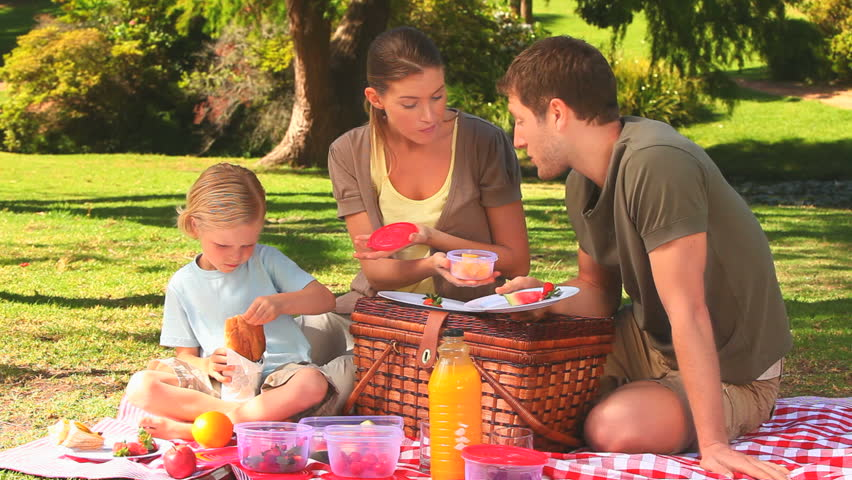
\includegraphics[scale = 0.35]{Sections/2StateOfTheArt/2_images/picinic.png}
        \caption{Generic picture of a family having a picnic.}
        \label{fig:picnic}  
    \end{figure}

    \begin{itemize}
        
        \item Computer output: Tree, bottle, person, apple, cup.
        \item Human output: A family having a picnic in the park.
    \end{itemize}
     
    \par A computer is only able to output the objects detected but it is incapable of giving them any sort of meaning.



%%%%%%%%%%%%%%%%%%%%%%%%%%%%%%%%%%%%%%%%%%%%%%%%%%%%%%%%%%%%%%%%%%%%%%%%%%%%%

    \subsection{Datasets With Common Objects}

    \label{dataset}

    \par A dataset is a collection of images and videos that contain every day life objects that are manually labeled. State-of-the-art object detection models require deep learning neural networks, and in order for neural networks to be trained, they  require training datasets, as previously explained.  

    \par A few examples of some available datasets are:  MS COCO \cite{Lin2014}, ImageNet \cite{Takamitsu1978} , VisualGenome \cite{Language2015}, OpenImages \cite{Kuznetsova2018} and Pascal-VOC \cite{Everingham2010}

    \par Some of these datasets propose challenges, where teams are able to compete in order to achieve state-of-the-art results. This subject is discussed in section \ref{sec:state}
    %%%%%%%%%%%%%%%%%%%%%%%%%%%%%%%%%%%%%%%%%%%%%%%%%%%%%%%%%%%%%%%%%%%%%%%%%%%%%%%%%%

%%%%%%%%%%%%%%%%%%%%%%%%%%%%%%%%%%%%%%%%%%%%%%%%%%%%%%%%%%%%%%%%%%%%%%%%%%%%%


\section{Computer Vision Libraries}
\label{sec:libraries}


%%%%%%%%%%%%%%%%%%%%%%%%%%%%%%%%%%%%%%%%%%%%%%%%%%%%%%%%%%%%%%%%%%%%%%%%%%%%%%%
    \subsection{OpenCV}

    OpenCV is an open source computer vision and machine learning software library originally developed by Intel in the year 2000 \cite{Culjak2012}.\par

    The library has more than 2500 optimized algorithms, which includes a comprehensive set of both classic and state-of-the-art computer vision and machine learning algorithms. These algorithms can be used to detect and recognize faces, identify objects, classify human actions in videos, track camera movements, track moving objects, extract 3D models of objects, produce 3D point clouds from stereo cameras, stitch images together to produce a high resolution image of an entire scene, find similar images from an image database, remove red eyes from images taken using flash, follow eye movements, recognize scenery and establish markers to overlay it with augmented reality, etc. \cite{opencvweb} \par
    
    OpenCV Supports the deep learning frameworks like Tensorflow, Torch/PyTorch, Caffe and it is the most standardized tooling for computer vision.  

    \subsubsection{Tensorflow}

    \label{Tensorflow}
   

    Tensorflow is currently the most popular open source framework for numerical computation and large-scale machine learning introduced by google and was originally created for tasks with heavy numerical computations.  \cite{Abadi} \cite{Dignam1983} 
    
    Tensorflow is written in c++ which enables extremely fast compile times, non the less, it can still be accessed by other languages, such as Python and also supports CPUs, GPUs and distributed processing. \par
    

    The name given to tensorflow comes from the inputs, since it receives inputs as a multi-dimensional array, also known as tensors. The input (tensor) goes on one end and then it “flows” throughout a system of operations and comes out on the other end as output. \par 
    
    Tensorboard is a feature of tensorflow that allows the monitoring of what tensorflow is doing graphical and visually.\par

%%%%%%%%%%%%%%%%%%%%%%%%%%%%%%%%%%%%%%%%%%%%%%%%%%%%%%%%%%%%%%%%%%%%%%%%%%%%%  
    \subsection{VLFeat}

    The VLFeat open source library implements popular computer vision algorithms specializing in image understanding and local features extraction and matching. Algorithms include Fisher Vector, VLAD, SIFT, MSER, k-means, hierarchical k-means, agglomerative information bottleneck, SLIC superpixels, quick shift superpixels, large scale SVM training, and many others. It is written in C for efficiency and compatibility, with interfaces in MATLAB for ease of use, and detailed documentation throughout. It supports Windows, Mac OS X, and Linux. \cite{vedaldi08vlfeat}

    \subsection{BOOFCV}

    BoofCV is an open source library written from scratch for real-time computer vision. Its functionality covers a range of subjects, low-level image processing, camera calibration, feature detection/tracking, structure-from-motion, fiducial detection, and recognition. \par
	BoofCV is organized into several packages: image processing, features, geometric vision, calibration, recognition,visualize, and IO. Image processing contains commonly used image processing functions which operate directly on pixels. Features contains feature extraction algorithms for use in higher level operations. \par Calibration has routines for determining the camera's intrinsic and extrinsic parameters. Recognition is for recognition and tracking complex visual objects. Geometric vision is composed of routines for processing extracted image features using 2D and 3D geometry. Visualize has routines for rendering and displaying extracted features. IO has input and output routines for different data structures \cite{boofcvweb}.

    \subsection{GluonCV}

    GluonCV provides implementations of state-of-the-art (SOTA) deep learning algorithms in computer vision. It aims to help engineers, researchers, and students quickly prototype products, validate new ideas and learn computer vision. \cite{Guo2019}

    
%%%%%%%%%%%%%%%%%%%%%%%%%%%%%%%%%%%%%%%%%%%%%%%%%%%%%%%%%%%%%%%%%%%%%%%%%

\section{Neural Networks}
\label{sec:neuralnet}

    \par A neural network can be considered a computer program that operates identically to how a human brain would, in the sense that it is able to be teachable to do certain tasks like problem-solving. The appeal of a neural network is the ability to emulate the human brain in pattern recognition skills. 


    \par Neural networks are composed of many small cells called neurons. These neurons are grouped into several layers that form columns. The connection between columns are formed also through their neurons. Each neuron of each layer is connected to another neuron of another layer. A visual representation of a generic neural network architecture is shown in figure \ref{fig:neural}.


    \begin{figure}[htb]
        \centering
        \includegraphics[scale = 0.5]{Sections/2StateOfTheArt/2_images/deeplearning.pdf}
        \caption{Typical neural network architecture. \cite{mathworks_NN}}
        \label{fig:neural}
    \end{figure}
        
    
    \par The connections between layers are called weighted connections and they are adjusted with a real-valued number attached to them. This number is important, because each neuron takes the value of the attached neuron (in their layer) and multiplies it by their connection weight. The bias value is an additional parameter in the neural network which is used to adjust the output along with weighted sum of the inputs to the neuron. The sum of the bias value with the weights  is put through an activation function which mathematically transforms the value and assigns it to the connected neuron in the adjacent layer. This is propagated through the whole network.  Se figure \ref{fig:neuron} for a clear representation of this process.
    

    
    \begin{figure}[htb]
        \centering
        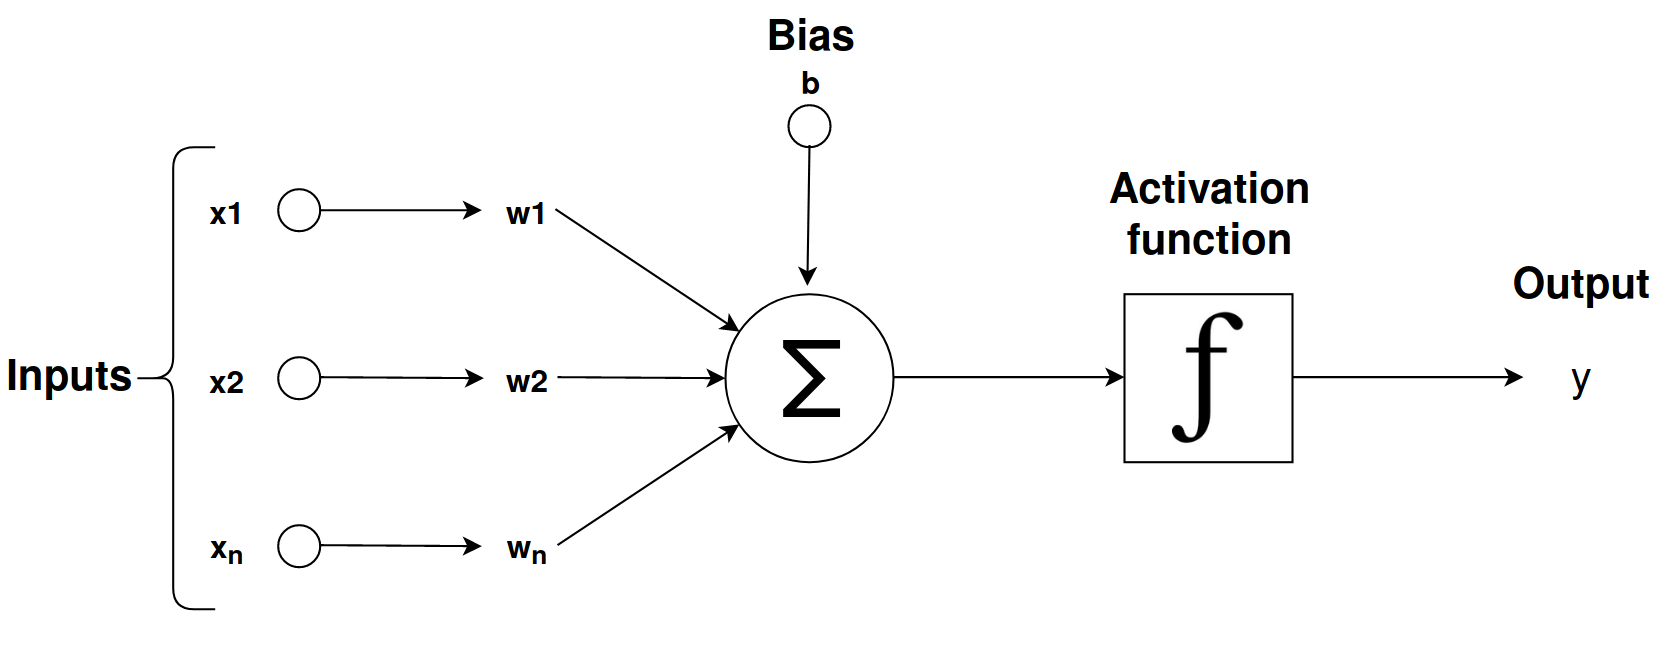
\includegraphics[scale = 0.15]{Sections/2StateOfTheArt/2_images/neuron.png}
        \caption{ Operations done by a neuron.}
        \label{fig:neuron}
    \end{figure}
    
    
   
    \par To put it simply, a neural network can be compared to a filter that goes through all of the possibilities, so that the computer is able to come up with the correct answer.
    \par Sometimes, an object might be too similar to another object which can make the network output a wrong answer. The solution to this problem is the usage of a back-propagation algorithm. This algorithm allows the network to adjust the connections back through the network, check if all the bias values are correct and all of the connections are weighted properly. \cite{ArmaanMerchant2018}
    


        \subsection{Neural Network Training}

        \par The best way to train a neural network from scratch is to design a network architecture that will learn through the feeding of a large dataset of labeled data. This allows it it to learn the features and model. The problem with this is that depending on the learning rate of the network and the amount of data, these networks can take a lot of time to train (days, maybe weeks). 

        \par To solve the problem of time, deep learning applications can recur to the usage of transfer learning. Transfer learning is a process that involves the fine-tuning of a pretrained model. This works by using an existing network like GoogLeNet, and feed it new data of previously unknown classes to the network. After some tweaks to the network, it will be able to categorize only a specific object instead of many different ones. This not only allows the network to be more precise in categorizing that one specific object, but it will also save lot of computation time.  \cite{mathworks_deeplearning}

        
        \subsection{Types of Neural Networks architectures}

            \subsubsection{Feedforward Neural Network}
            
            \par A Feedforward neural network has the most simple architecture, the data only travels in one single direction. It goes through the input node and exits at the output node. Since there is no back-propagation algorithm this neural network is not able to correct itself. \cite{ArmaanMerchant2018}

            \begin{figure}[htb]
                \centering
                \includegraphics[scale = 0.75]{Sections/2StateOfTheArt/2_images/neural-network.pdf}
                \caption{ Example of a Feedforward Neural Network with one hidden layer (with 5 neurons) \cite{neural_image}. }  
            \end{figure}

            \newpage
            \subsubsection{Radial Basis Function Neural Network}

            \par This network is composed of two layers. In the first one features are combined with a radial basis function in the inner layer. The second one is the output, where these features are taken in consideration while computing the same output in the next function.
            \par A radial basis function means that the distance of a point is considered with respect to the center. \cite{ArmaanMerchant2018}


            \subsubsection{Recurrent Neural Network (RNN)} 

            \par Recurrent Neural Networks (RNNs) are designed to recognize sequential data characteristics and use patterns to predict the next likely scenario. In these kind of neural networks the signals are propagated in both directions as well as within the layers. They work on the principle of saving the output of a layer and feeding it to the input to help in the prediction of the outcome of the layer.
            \par RNNs use the back-propagation algorithm which allows to make sure that the output is correct almost 100\% of the time. \cite{ArmaanMerchant2018}
        


            \subsubsection{Convolutional Neural Network (CNN)}
            
            \par CNNs, also known as ConvNets, are a class of deep neural networks that employ the mathematically convolutional operation in at least one of its layers and have a deep feed-forward (not recurrent) architecture \cite{Ribeiro}. They share similarities with feedforward neural networks, since neurons also have weights and biases that are able to learn. In this network the input features are taken like a filter, which allows the network to have memory, since it can remember the images in parts and compute operations like conversion of the image from RGB or HSI to grayscale, allowing the detection of edges and images that can be classified into different categories. \cite{ArmaanMerchant2018}

            \par The only notable difference between CNNs and traditional ANNs is that CNNs are primarily used in the field of pattern recognition within images. This allows the encoding image-specific features into the architecture, making the network more suited for image-focused tasks, while further reducing the parameters required to set up the model. \cite{OShea2015}
            
            

            \par CNN convolves learned features with input data, and uses 2D convolutional layers which make this architecture one of the best to process 2D data, such as images. They also remove the necessity of manual feature extraction. There is no need to identify features used to classify images since CNNs work by extracting them directly from images. This is important because relevant features are not pretrained, they are learned while the network trains on a dataset. \cite{mathworks_deeplearning}

            \begin{figure}[htb]
                \centering
                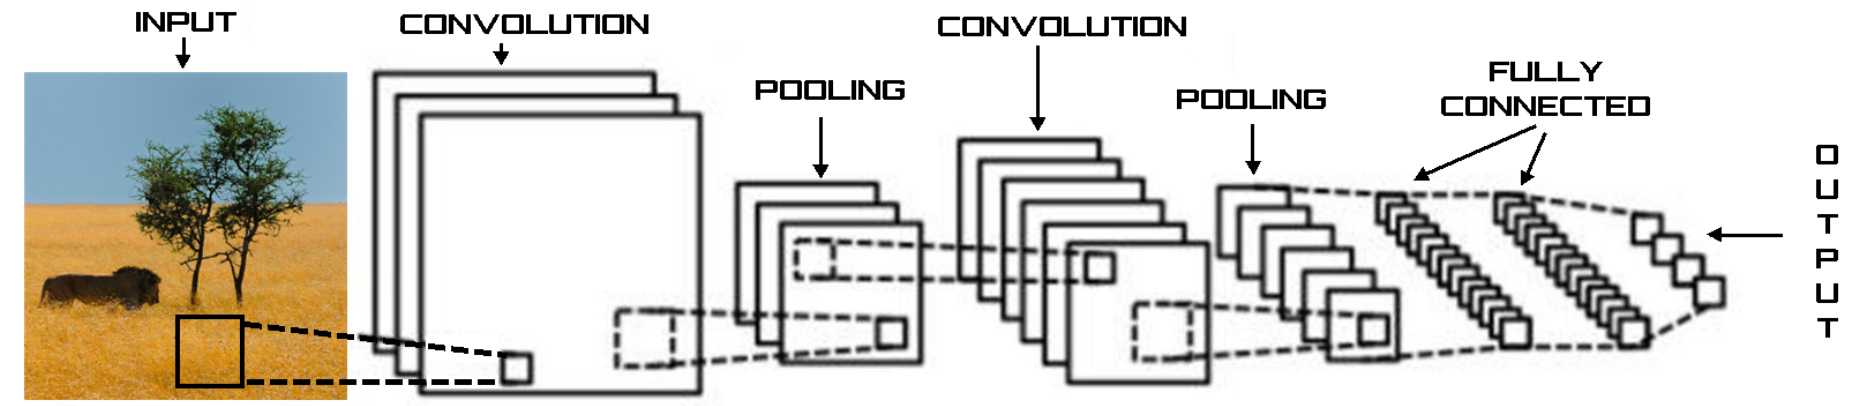
\includegraphics[scale = 0.17]{Sections/2StateOfTheArt/2_images/conv.png}
                \caption{CNN architecture }  \cite{Ribeiro}
            \end{figure}

            
           \par \textbf{Input Layers}
           \par The input layer is the first layer of a CNN and serves the purpose of resizing an image in order for it  to pass onto further layers for feature extraction \cite{Ribeiro}. It also holds the pixel value of the images \cite{OShea2015}. \bigbreak
            
          
           \par \textbf{Convolutional Layers}
           \par The convolutional layers extracts low-level features from an image, such as edges, color or gradient orientation, according to the applied filter or kernel. \cite{Ribeiro} \bigbreak

           \par \textbf{Activation Functions}
           \par The activation function introduces nonlinearity in order for CNNs to learn functionalities. They serve as decision functions and help in learning complex patterns. Some examples of activation functions are sigmoid, softmax and ReLU. \cite{Ribeiro} \bigbreak

           \par \textbf{Pooling Layers} 
           \par The pooling layers serve the purpose of reducing the parameters required and computation in the network by controlling the overfitting. This is achieved by reducing the spatial size of the network. \cite{Ribeiro}
           \par Overfitting happens when a model learns the detail and noise in the training data to an extent that it negatively impacts the performance of the model on new data. \cite{OShea2015} \bigbreak


           \par \textbf{Fully Connected Layers}
            \par  The final layer in a CNN is usually a fully connect layer used for classification purposes. They take all features from the previous layer and compute class probabilities or scores. These features are then translated into a different class. \cite{Ribeiro} \bigbreak
            
            
%%%%%%%%%%%%%%%%%%%%%%%%%%%%%%%%%%%%%%%%%%%%%%%%%%%%%%%%%%%%%%%%%%%%%%%%%
\section{CNNs architectures For Image Classification}
\label{sec:cnn}
    \subsection{SquezeeNet}
    \label{SquezeeeNet}

    SquezeeNet is a deep neural network for computer vision that is more efficient for distributed training, since it requires less parameters to be transferred. The main goal of SquezeeNet creation was to obtain a smaller neural network with fewer parameters that could more easily fit into a computer memory, making it more easily transmitted over a computer network. This neural network was firstly implemented on top of the caffe deep learning software framework and later ported to the chainer deep learning software framework and Apache MXNET framework.\par
    The basis of SquezeeNet consists on 3 ideas \cite{Iandola2016}:

    \begin{itemize}
        \item Replacing 3x3 filters with 1x1 filters and reduce the number of input channels. This improves computation speed and alleviates the computer resources required, since 1x1 filters have 9 times less parameters than 3x3 filters.
        \item Utilize 1x1 filters as a bottleneck layer to help reducing the computation required for the following 3x3 filters.
        \item Keeping a big feature map by down sampling late.
    \end{itemize}

    

    This neural network is built with fire modules, which are represented in figure \ref{fig:firemodule}. 


    \begin{figure}[htb]
        \centering
        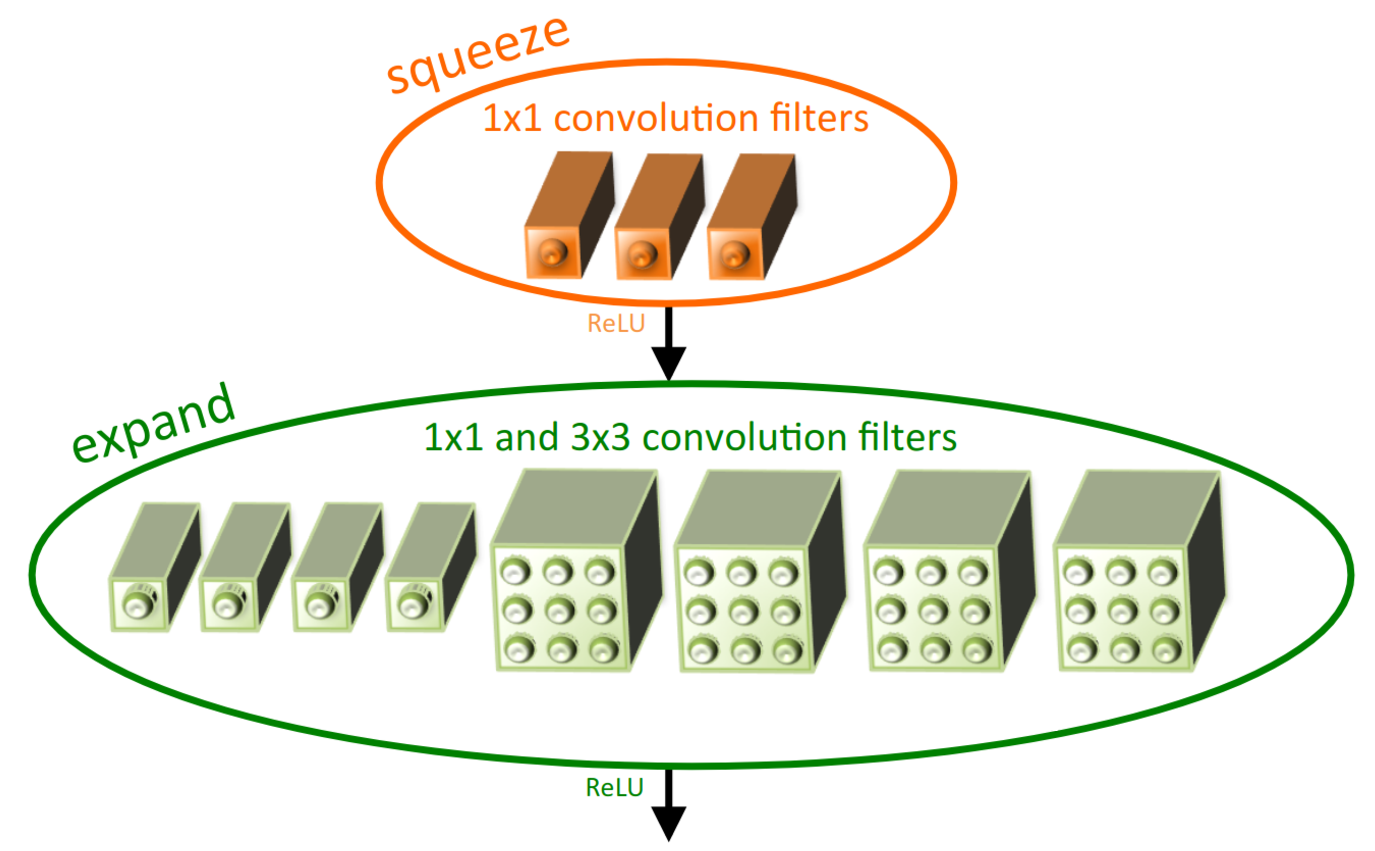
\includegraphics[scale = 0.17]{Sections/2StateOfTheArt/2_images/firemodule.png}
        \caption{SqueezeNet fire module. \cite{Iandola2016} }  
        \label{fig:firemodule}
    \end{figure}

    The fire module contains both a squeeze layer and an expand layer. SquezeeNet stacks fire modules and pooling layers  (this can be seen in figure \ref{fig:squezeenet}). The squeeze layer and expand layer maintain the same feature map size, while the pooling layers reduce the depth to a smaller number, later increasing it. Reducing the depth means the expand layer has fewer computations to do, boosting the speed.\par


    \hfill
    
   \textbf{Squeeze layer architecture: } Consists on 1x1 convolutions, it essentially combines all the channels of the input data into one (and thus reducing the number of input channels needed in the next layer).\par
   \hfill

   \textbf{Expand layer architecture:} Consists on 1x1 convolutions mixed alongside 3x3 convolutions. The 1x1 convolutions combine the channels of the previous layers in various ways. The 3x3 convolutions detect structures in the image since 1x1 convolutions can’t. \par
   \hfill

   \textbf{SquezeeNet architecture:} SquezeeNet doesn’t fully connect layers and it consists of 8 fire modules and a single convolution's layer as input and output. It uses Global Average Pooling, taking each channel from the previous convolution layer and builds an average over all values.



   \begin{figure}[htb]
    \centering
    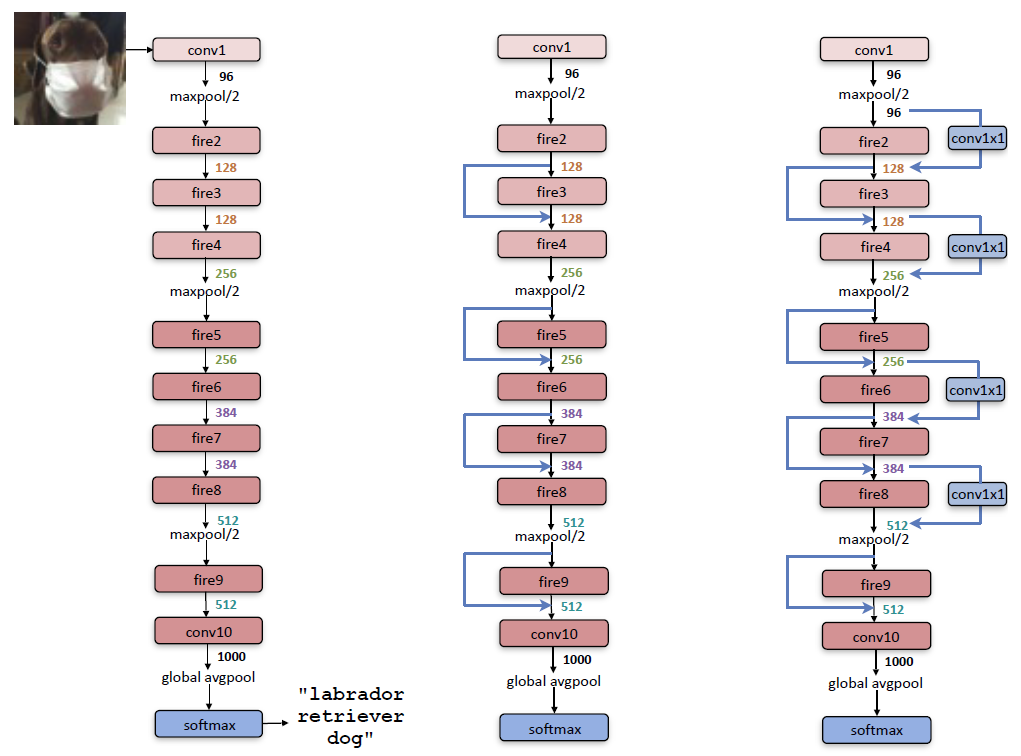
\includegraphics[scale = 0.3]{Sections/2StateOfTheArt/2_images/squezeeNetArchitecture.png}
    \caption{SqueezeNet architecture. \cite{squeezenetweb}} 
    \label{fig:squezeenet}
\end{figure}


   
    \newpage
    
%%%%%%%%%%%%%%%%%%%%%%%%%%%%%%%%%%%%%%%%%%%%%%%%%%%%%%%%%%%%%%%%%%%%%%%%%%%%%

    \subsection{ResNet}

    The core idea of ResNet (Residual Neural Network) is introducing skip connections (also called identity shortcut connection, represented in figure \ref{fig:skip}). The way this works is by adding the output of an earlier layer to a later layer in order to jump over some layers. \par

    The vanishing of gradients problem makes deep neural networks hard to train, this happens because as the gradient is propagated back to earlier layers, repeated multiplications may turn the gradient too small, this results in a rapidly performance degradation. \par
    
    Skipping over layers helps avoiding the vanishing of gradients problem and improves the accuracy of the neural network. \par

    Having the skip connection allows the training of extremely deep neural networks, more than 150 layers, successfully and still being able to 
    achieve a compelling performance. \cite{He2016} \par
    \par This architecture is represented in figure \ref{fig:resnet}.
    \begin{figure}[htb]
        \centering
        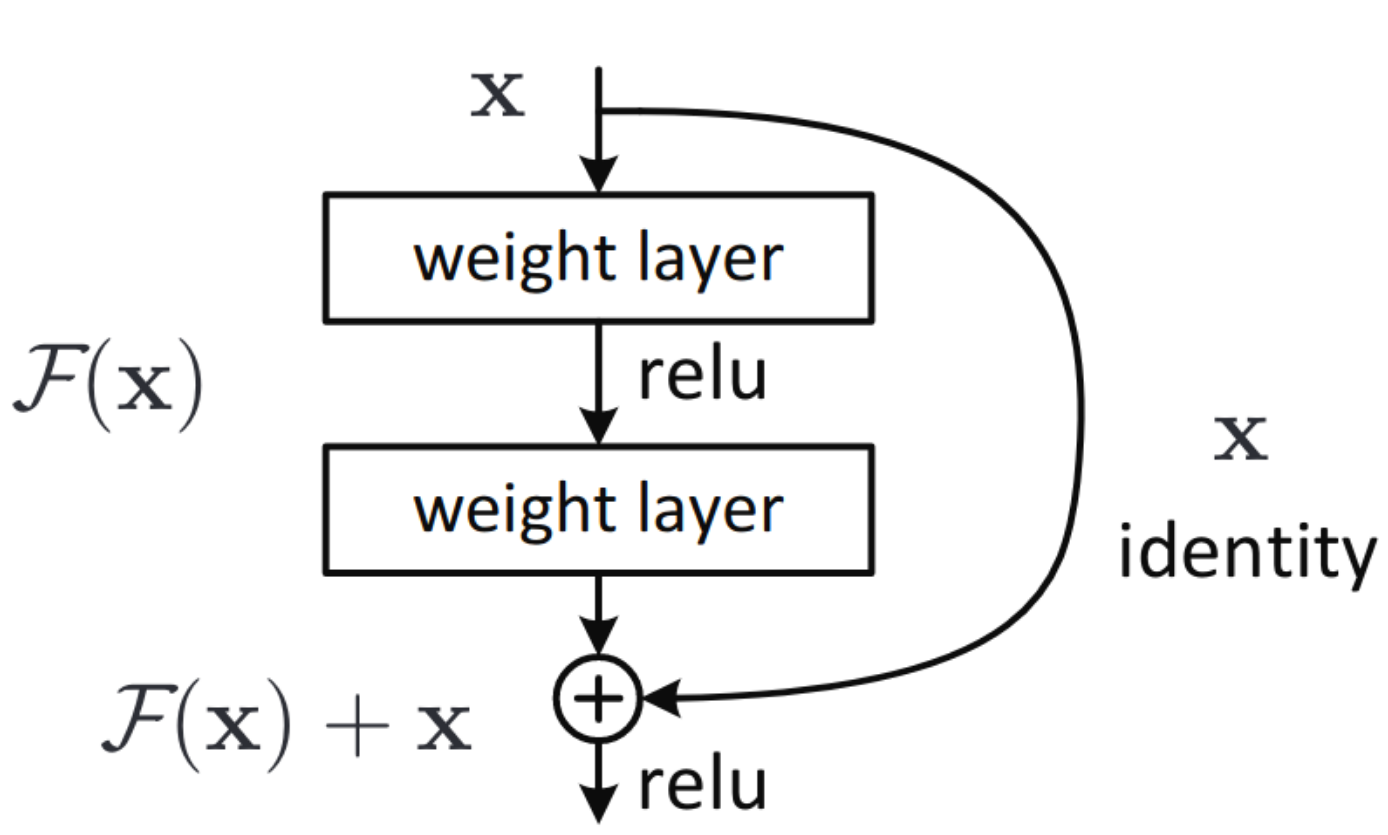
\includegraphics[scale = 0.12]{Sections/2StateOfTheArt/2_images/resnet_block.png}
        \caption{Skipping connection example.\cite{He2016}} 
        \label{fig:skip}
    \end{figure}

    

    \begin{figure}[htb]
        \centering
        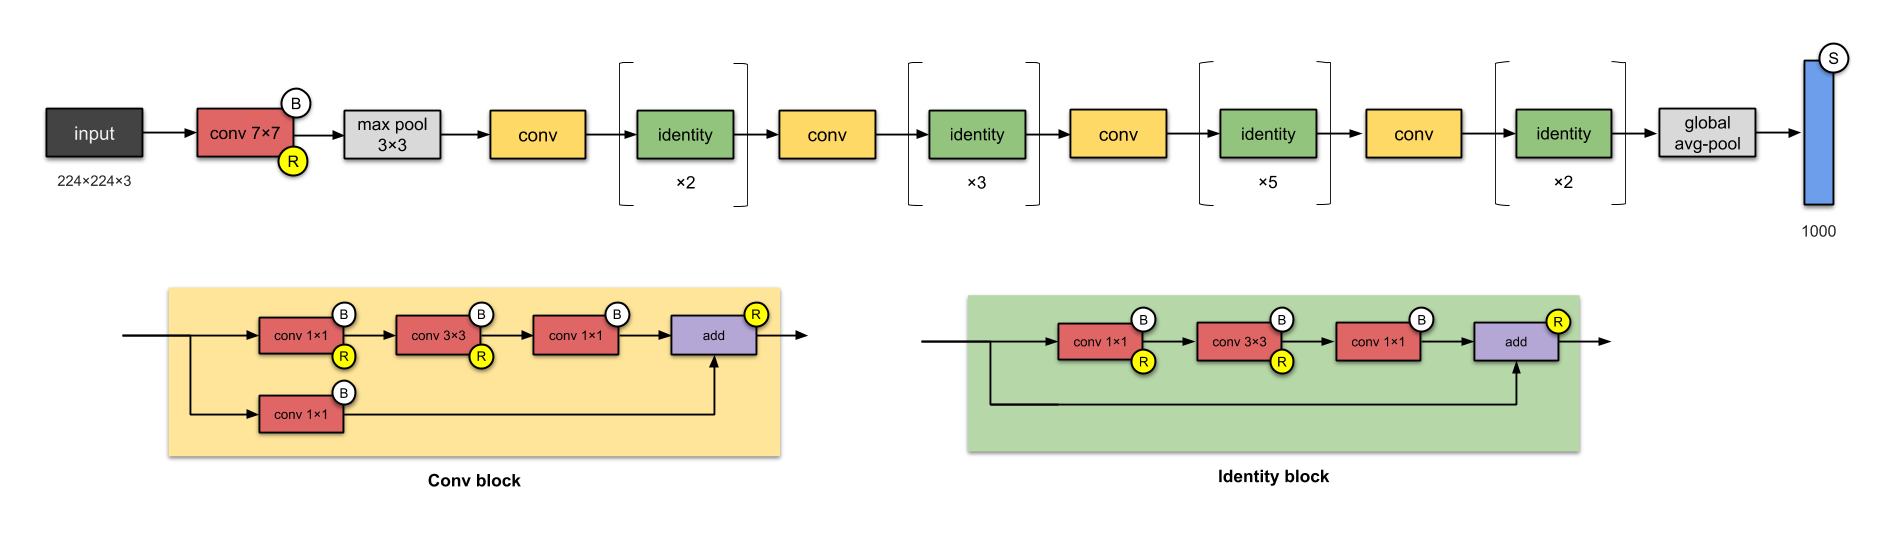
\includegraphics[scale = 0.22]{Sections/2StateOfTheArt/2_images/resnet_arch.png}
        \caption{ResNet Architecture.\cite{cnnarchitectures}} 
        \label{fig:resnet}
    \end{figure}

\newpage
%%%%%%%%%%%%%%%%%%%%%%%%%%%%%%%%%%%%%%%%%%%%%%%%%%%%%%%%%%%%%%%%%%%%%%%%%%%%%

    \subsection{InceptionV3}

    \par Initially named GoogLeNet, the Inception-v1 architecture was proposed by researchers of Google company and was the winner of the ILSVRC 2014 competition, making it historically significant in Convolutional Neural Networks. 
    \par This network, trained on the imageNet dataset, introduced inception modules (shown in figure \ref{fig:inception_module}) that allowed for a more efficient computation and deeper network.

    \begin{figure}[htb]
        \centering
        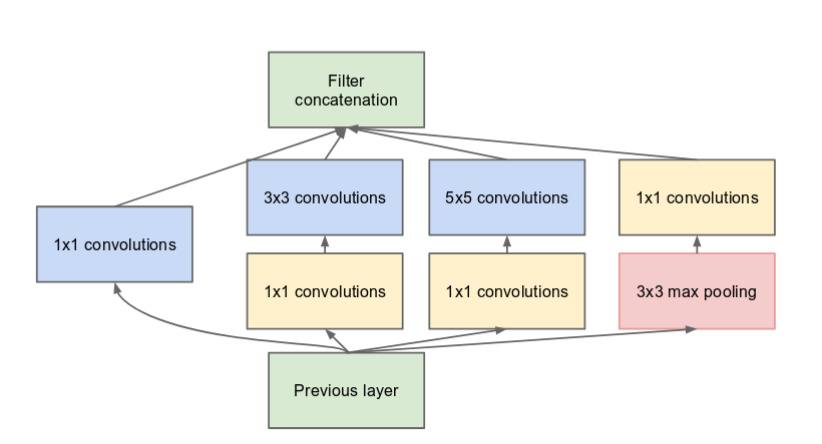
\includegraphics[scale = 0.35]{Sections/2StateOfTheArt/2_images/inceptionArchitecture.png}
        \caption{Inception Module. \cite{inceptionV3web2}} 
        \label{fig:inception_module}
    \end{figure}

    \par The Inception architecture (Inception-v1) was improved by the introduction of batch normalization (Inception-v2). \cite{Ribeiro}


    InceptionV3, is 48 layers deep and able to classify images into 1000 different categories. The improvement over its predecessors is the adding of factorization ideas (figure \ref{fig:factorization} shows an example of this). 

    \begin{figure}[htb]
        \centering
        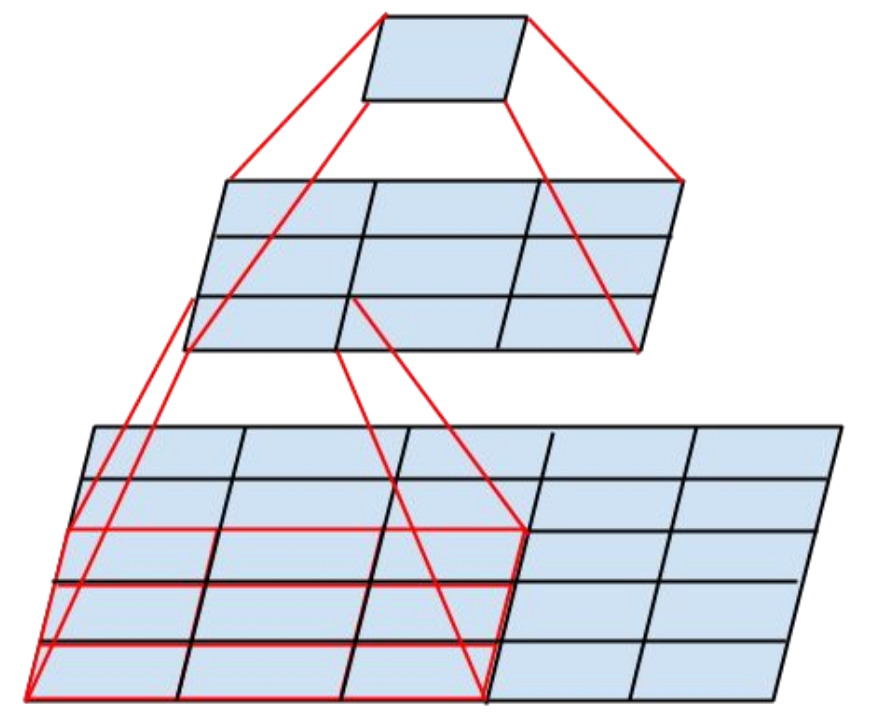
\includegraphics[scale = 0.15]{Sections/2StateOfTheArt/2_images/factor_inception.png}
        \caption{Mini-network replacing the 5×5 convolutions (Example of factorization). \cite{Szegedy2016}} 
        \label{fig:factorization}
    \end{figure}


    \par This third interaction aims at factorizing convolutions, reducing the number of connections/parameters required while maintaining network efficiency. As an example, using a layer of 5x5 filter requires 5x5=25 parameters, this layer can be replaced by two 3x3 layers which reduce the number of parameters required by 28\%, since 2x(3x3) = 18 parameters. Reducing the number of parameters required reduces the computational resources required and also prevents overfitting. This enables the network to go deeper. \cite{inceptionV3web} 
    \par The inceptionv3 architecture can be seen in figure  below.
  
    \begin{figure}[htb]
        \centering
        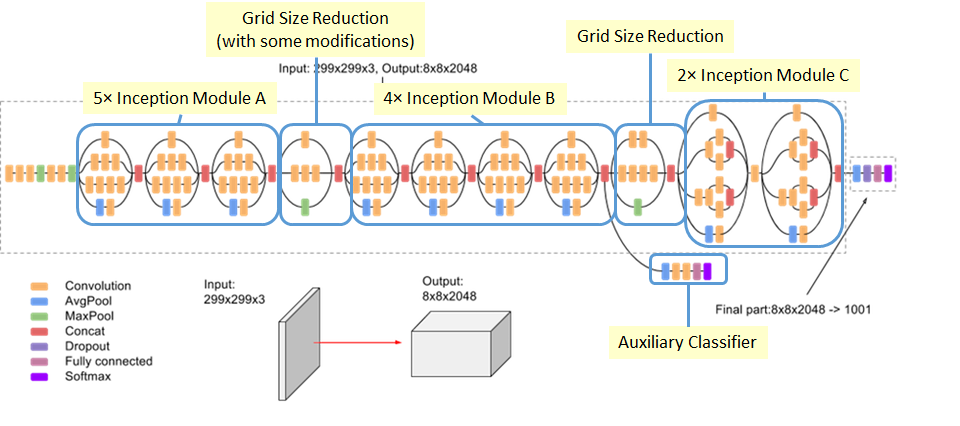
\includegraphics[scale = 0.4]{Sections/2StateOfTheArt/2_images/inceptionv3_architecture.png}
        \caption{InceptionV3 architecture.\cite{inceptionV3web}} 
    \end{figure}

    \par Even though InceptionV4 \cite{szegedy2016inceptionv4} is already available it was not used in this work. The improvements over its predecessor are as follow: 
    \begin{enumerate}
        \item Converting Inception modules to Residual Inception blocks.
        \item Adding more Inception modules.
        \item Adding a new type of Inception module (Inception-A) after the Stem module.
    \end{enumerate}
    
    
    
   

    \newpage
%%%%%%%%%%%%%%%%%%%%%%%%%%%%%%%%%%%%%%%%%%%%%%%%%%%%%%%%%%%%%%%%%%%%%%%%%%%%%
    \subsection{DenseNet}

    Densely Connected Convolutional Networks aim at expanding the depth of deep convolutional networks by connecting each layer to every other layer, in a feed forward fashion (this can be seen in figure \ref{fig:densenet}), this reduces  the number of parameters required, and alleviates the problem of the vanishing-gradients, while improving feature propagation (ensuring maximum information and gradient flow) and feature reuse which allows the learning of more compact and accurate models. This kind of neural network simplifies the connectivity pattern between layers introduced in other architectures (such as ResNets). \cite{Szegedy2016} \par

    The improved flow of information and gradients makes DenseNets easier to train, since each layer has direct access to the gradients from the loss function and the original input signal, leading to an implicit deep supervision. \par

    DenseNets scale naturally to hundreds of layers, while exhibiting no optimization difficulties.


    \begin{figure}[htb]
        \centering
        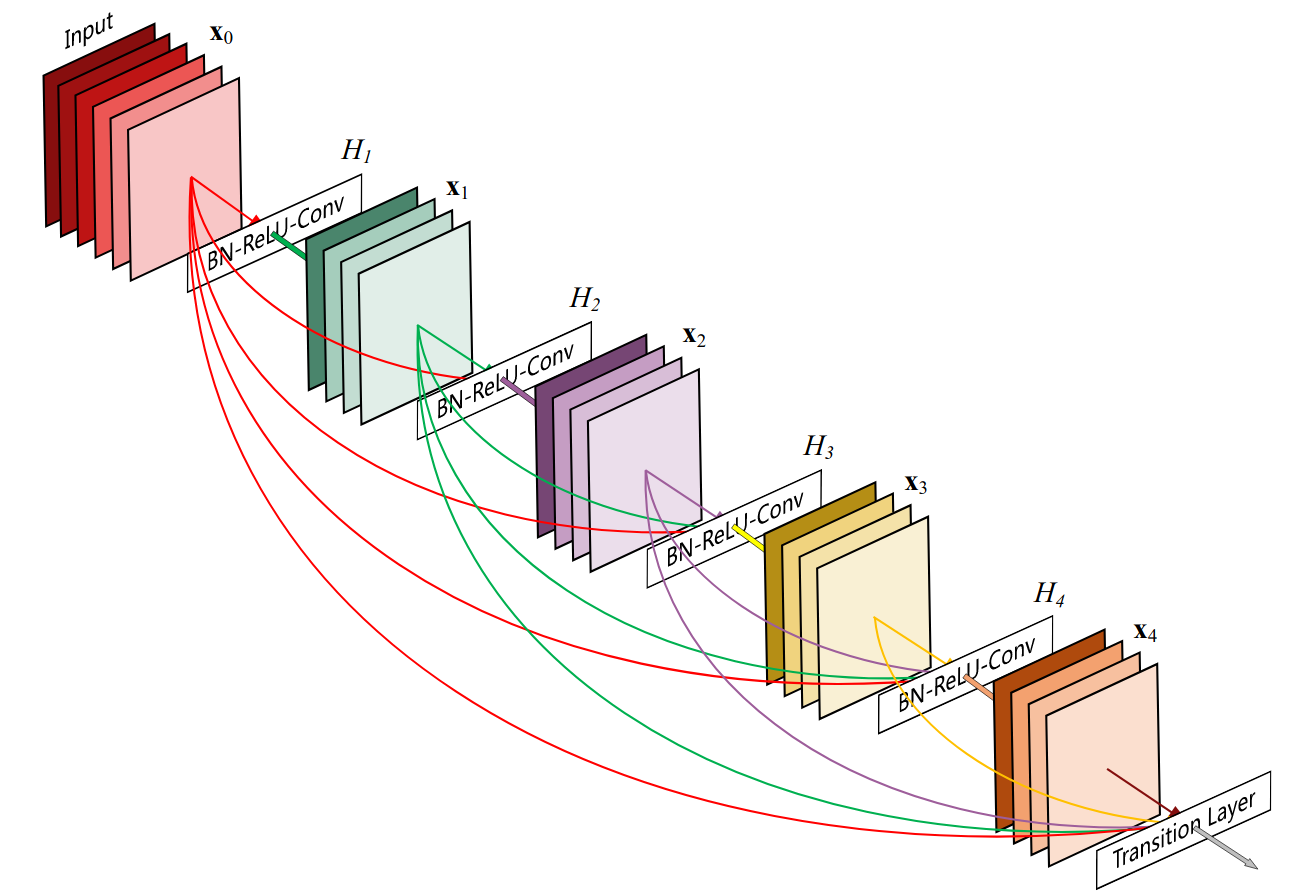
\includegraphics[scale = 0.15]{Sections/2StateOfTheArt/2_images/denseNet.png}
        \caption{A 5-layer dense block. Each layer takes all preceding feature-maps as input. \cite{Szegedy2016} } 
        \label{fig:densenet}
    \end{figure}
    

%%%%%%%%%%%%%%%%%%%%%%%%%%%%%%%%%%%%%%%%%%%%%%%%%%%%%%%%%%%%%%%%%%%%%%%%%%%%%


\section{Regression based algorithms for Object Detection}
\label{sec:regression}
\par Regression based algorithms (also called single stage detectors) work differently than classification based algorithms. Instead of selecting multiple interesting parts of an image, they predict classes and bounding boxes for the entire image in one single run of the algorithm.
\par These algorithms are extremely fast but are not so accurate as classification based algorithms. \cite{Lin2017} 
RetinaNet, YOLO and SSD are a few examples of object detection algorithms of this type. \par


%%%%%%%%%%%%%%%%%%%%%%%%%%%%%%%%%%%%%%%%%%%%%%%%%%%%%%%%%%%%%%%%%%%%%%%%%%%%%
    \subsection{RetinaNet}

    RetinaNet is a one-stage object detector presented at the 2017 International Conference on Computer Vision by the Facebook AI Research.\par

    In order to improve performance a loss function was implemented, called Focal Loss, allowing the network to focus more on difficult samples. With the loss function, alongside a one-stage network architecture, RetinaNet is able to achieve state-of-the-art performance in terms of accuracy and running time.\par

    This neural network is essential composed of one backbone network and two subnetworks. The backbone network is called Feature Pyramid Net \cite{lin2016feature}, built on top of ResNet, and has the purpose of computing convolutional feature maps of an image. Both subnetworks serve different purposes, one is for object classification using the backbone network output and the other subnetwork is responsible for performing the bounding box regression using the backbone network output.\cite{Lin2017} \par

    In figure \ref{fig:retinanet} its observable the Feature Pyramid Network (FPN) on top of the convolutional neural network ResNet as a backbone network (a) to generate a rich convolutional feature pyramid (b). The class subnet (c) is for classifying anchor boxes, and the box subnet (d) is for regressing from anchor boxes to ground-truth object boxes. \par 


    \begin{figure}[htb]
        \centering
        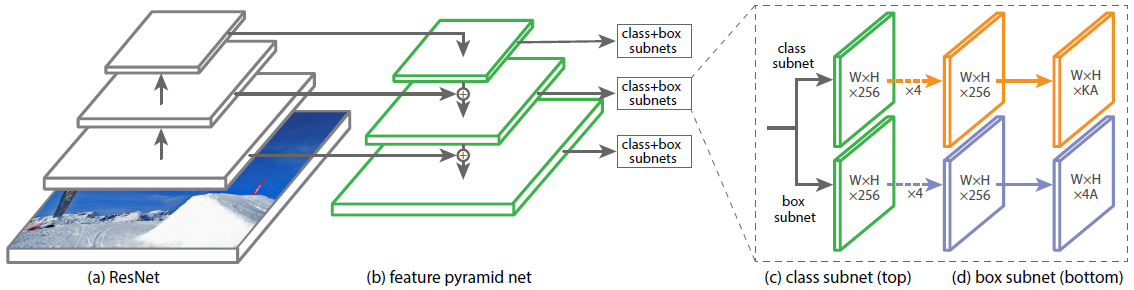
\includegraphics[scale = 0.37]{Sections/2StateOfTheArt/2_images/RetinaNet.png}
        \caption{RetinaNet architecture.\cite{Lin2017}} 
        \label{fig:retinanet}
    \end{figure}

%%%%%%%%%%%%%%%%%%%%%%%%%%%%%%%%%%%%%%%%%%%%%%%%%%%%%%%%%%%%%%%%%%%%%%%%%%%%%

    \subsection{YOLOv3}

    YOLOV3 (You Only Look Once Version 3) is a state-of-the-art, real-time object detection that’s in the third iteration of the original YOLO, it’s extremely fast and accurate (on par with the accuracy of focal loss from RetinaNet, but 4 times faster). YOLO allows the user to tradeoff between speed and accuracy simply by changing the size of the model.\par

    Compared to other classification networks that perform predictions multiple times for various regions in an image, YOLO architecture is more like a fully convolutional neural network do to the fact that it takes an image as input and passes it only once through the FCNN. The network divides the image into regions and predicts bounding boxes (weighted by predicted probabilities) and probabilities to each region, outputting a vector of bounding boxes and classes predictions. \par 
    
    \par YOLO works by dividing an image in an SxS grid and assuming B bounding boxes per grid. Each of the bounding box predicts 4 coordinates, object and class probabilities. \cite{Agarwal2019}

    \begin{figure}[htb]
        \centering
        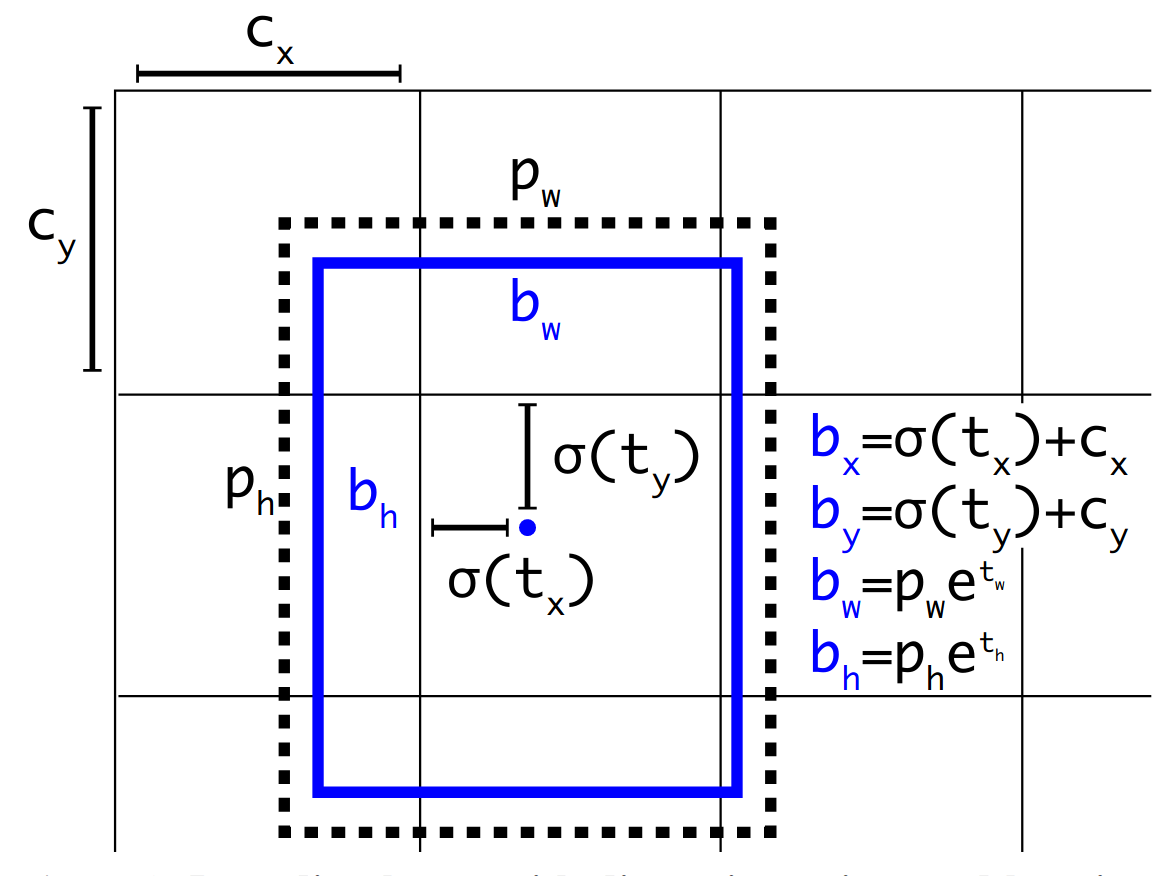
\includegraphics[scale = 0.13]{Sections/2StateOfTheArt/2_images/yolo_boundingbox.png}
        \caption{Bounding Box Prediction : Predicted Box (Blue), Prior Box (Black Dotted).\cite{Redmon2018}} 
    \end{figure}

    \newpage
    \par YOLO image predictions are informed by global context in the image since it can look at the entire image at the test time. This gives it several advantages over classifier-based systems. In addition, this algorithm also uses an open source neural network called Darknet-53 for feature extraction, this neural network is written in C and CUDA and it supports CPU and GPU computation. \cite{Redmon2018}\par 
    \par The full architecture of YOLOv3 is represented in figure \ref{fig:yolov3}.

    \begin{figure}[htb]
        \centering
        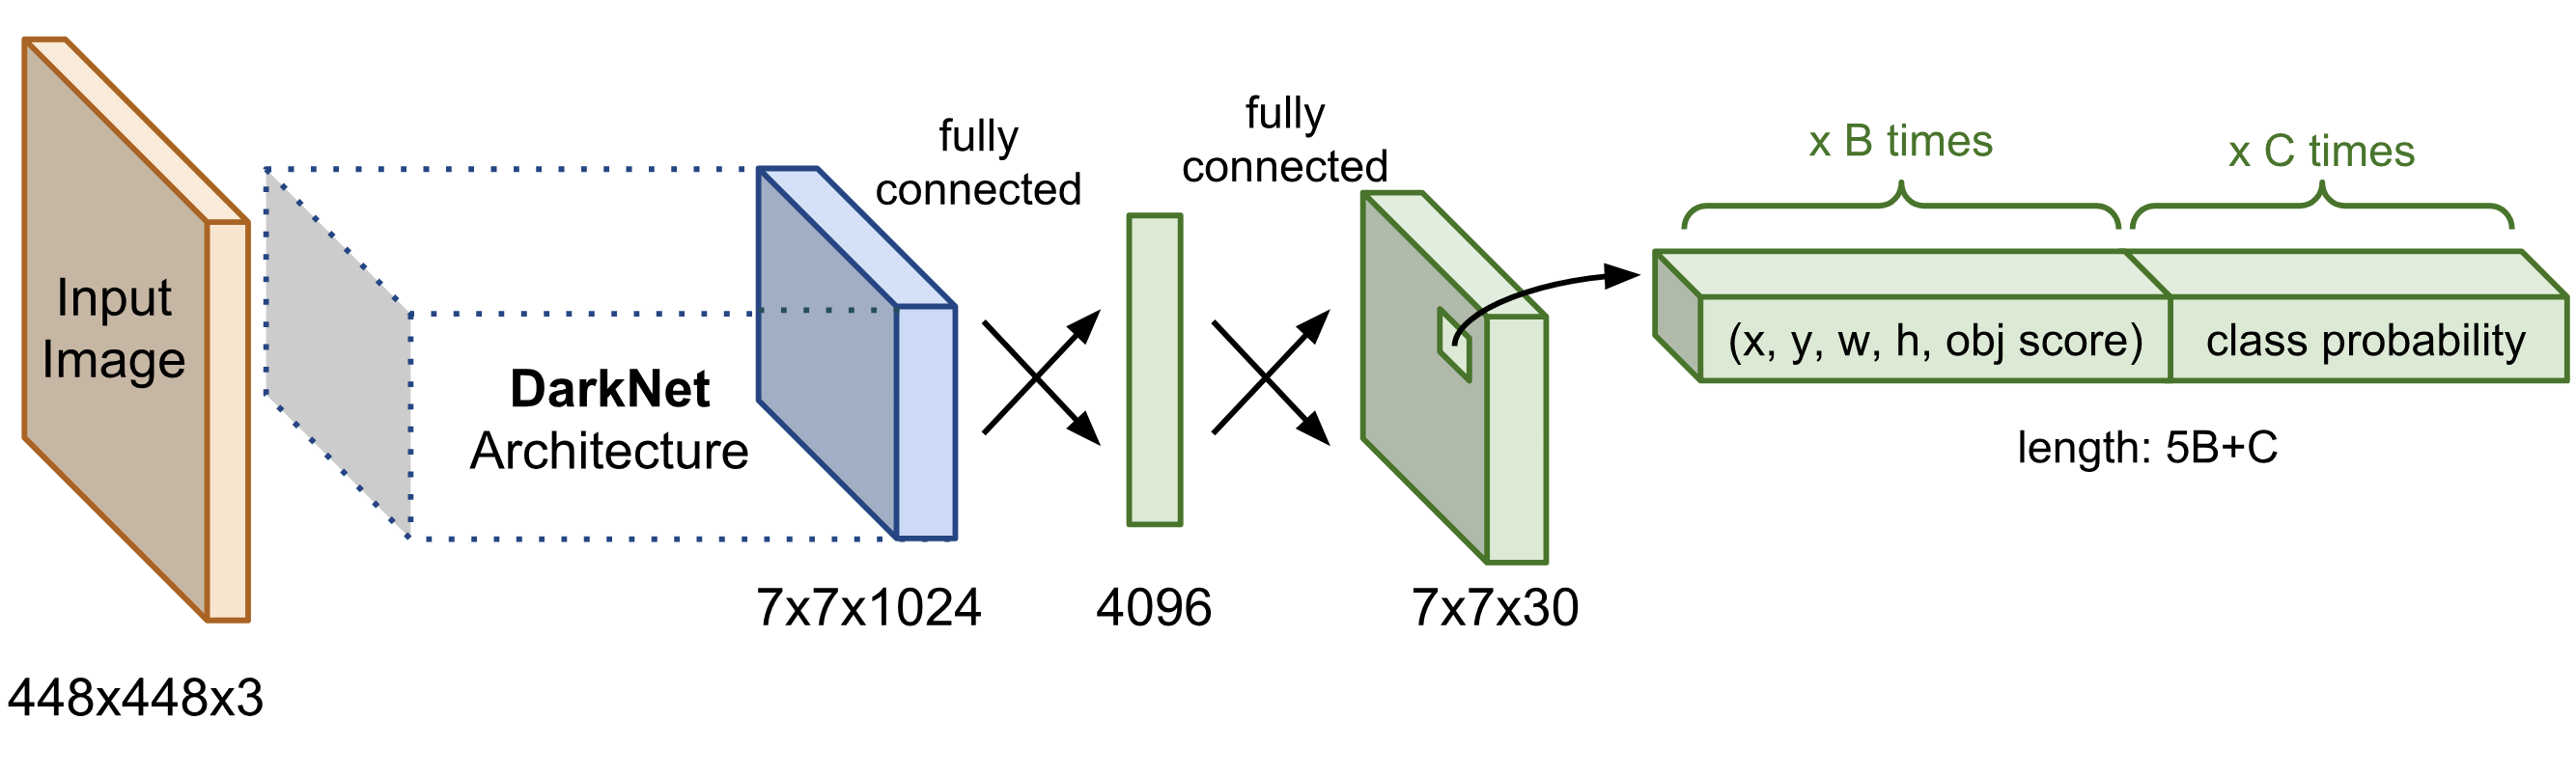
\includegraphics[scale = 0.26]{Sections/2StateOfTheArt/2_images/yolo-network-architecture.png}
        \caption{The network architecture of YOLO base model.\cite{weng2018detection4} }
        \label{fig:yolov3} 
    \end{figure}

    

   

%%%%%%%%%%%%%%%%%%%%%%%%%%%%%%%%%%%%%%%%%%%%%%%%%%%%%%%%%%%%%%%%%%%%%%%%%%%%%%%

    \subsection{TinyYoloV3}

    TinyYOLOv3 is a smaller model of YOLOv3 that requires less computational resources since it doesn’t occupy a large amount of memory , making it able to run in a smartphone. This model has a smaller number of convolutional layers, which improves the detection for small targets, therefore, it’s a model best suited for constrained environments. In its architecture this network is composed of 7 convolutional layers and 6 pooling layers and can detect 80 different object categories.  For complex scenes TinyYOLO is not accurate enough, however it is one of the fastest algorithms available. \cite{Yi2019}


    \subsection{Single Shot MultiBox Detector (SSD)}

    %%%%
    
    \par SSD is a method for detecting objects in images using a single deep neural network. This Multibox detector discretizes the output space of bounding boxes into a set of default boxes over different aspect rations and scales per feature map location.

    \par The base network of SSD is a VGG-16 network \cite{simonyan2014deep} followed by multibox convolutional layers. VGG-16 has the purpose of extracting the features for high quality image classification. The additional convolutional layers have the purpose of detecting objects, they are located at the end of the base network and decrease in size progressively, which helps with the detection of objects at multiple scales. The deep layers cover larger receptive fields and are helpful for larger objection detection, while the initial convolutional layers cover smaller receptive fields and are used for smaller objects detection. \cite{Liu2016}
    \par The added auxiliary structure can be summarized in the following key points:

    \begin{itemize}
        \item \textbf{Multi-scale feature maps for detection}. These layers decrease in size progressively and allow predictions of detections at multiple scales.
        \item \textbf{Convolutional predictors for detection}. Each added feature layer can produce a fixed set of detection predictions using a set of convolutional 
        filters.
        \item \textbf{Default boxes and aspect ratios}. They associate a set of default bounding boxes with each feature map cell, for multiple feature maps at the top of the network. The default boxes tile the feature map in a convolutional manner, so that the position of each box relative to its corresponding cell is fixed.
    \end{itemize}

    
    \par The SSD architecture is represented in figure \ref{fig:ssd}.

    \begin{figure}[htb]
        \centering
        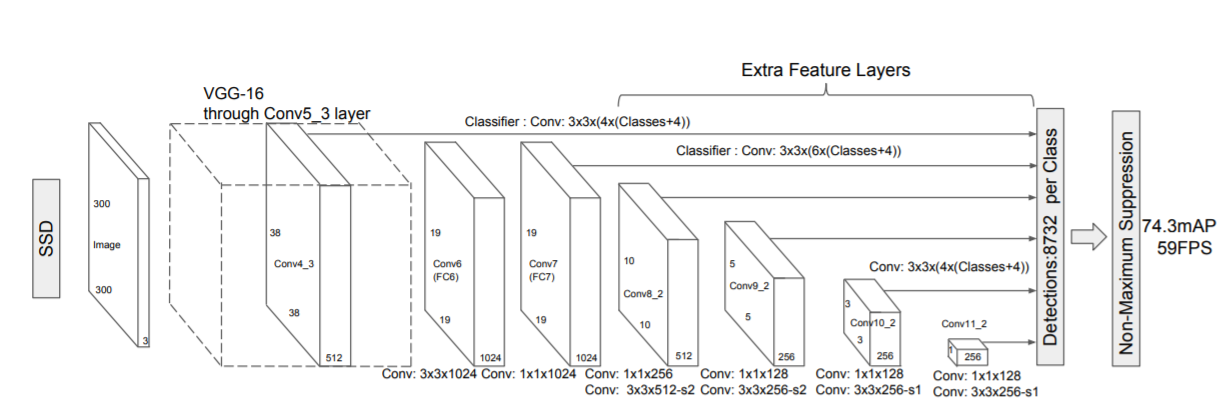
\includegraphics[scale = 0.35]{Sections/2StateOfTheArt/2_images/ssd_arch.png}
        \caption{SSD architecture. \cite{Liu2016}} 
        \label{fig:ssd}
    \end{figure}



    \par The prediction of bounding boxes is done by multiple feature maps of different sizes that represent multiple scales. During prediction time, the network generates scores for the presence of each object category in each default box and produces adjustments to the box to better match the object shape. The network also combines predictions from multiple feature maps with different resolutions to naturally handle objects of various sizes.
    \par SSD is simple relative to methods that require object proposals because it completely eliminates proposal generation and subsequent pixel or feature resampling stages and encapsulates all computation in a single network. This makes SSD easy to train.
    \par The core of SSD is predicting category scores and box offsets for a fixed set of default bounding boxes using small convolutional filters applied to feature maps.
    \par To achieve high detection accuracy, SSD produces predictions of different scales from feature maps of different scales, and explicitly separate predictions by aspect ratio.
    \par These design features lead to simple end-to-end training and high accuracy, even on low resolution input images, further improving the speed vs accuracy trade-off.
    \par This approach is based on a feed-forward convolutional network that produces a fixed-size collection of bounding boxes and scores for the presence of object class instances in those boxes, followed by a non-maximum suppression step to produce the final detections. \cite{Liu2016}
   
   

\section{Classification Based Algorithms For Object Detection}
\label{sec:classification}

\par Classification based algorithms work in two stages. Firstly, they select interesting regions from the image and secondly, they classify those regions using convolutional neural networks. The problem with this approach is that it can be extremely slow since a prediction is run for every selected region, however this approach is extremely accurate. \cite{Lin2017} 
\par RCNN, Fast-RCNN and Faster-RCNN are some types of classification based algorithms.  

    \subsection{R-CNN Models Summary}

    \par In the picture below a  compact summary of all of the R-CNN models.

    \begin{figure}[htb]
        \centering
        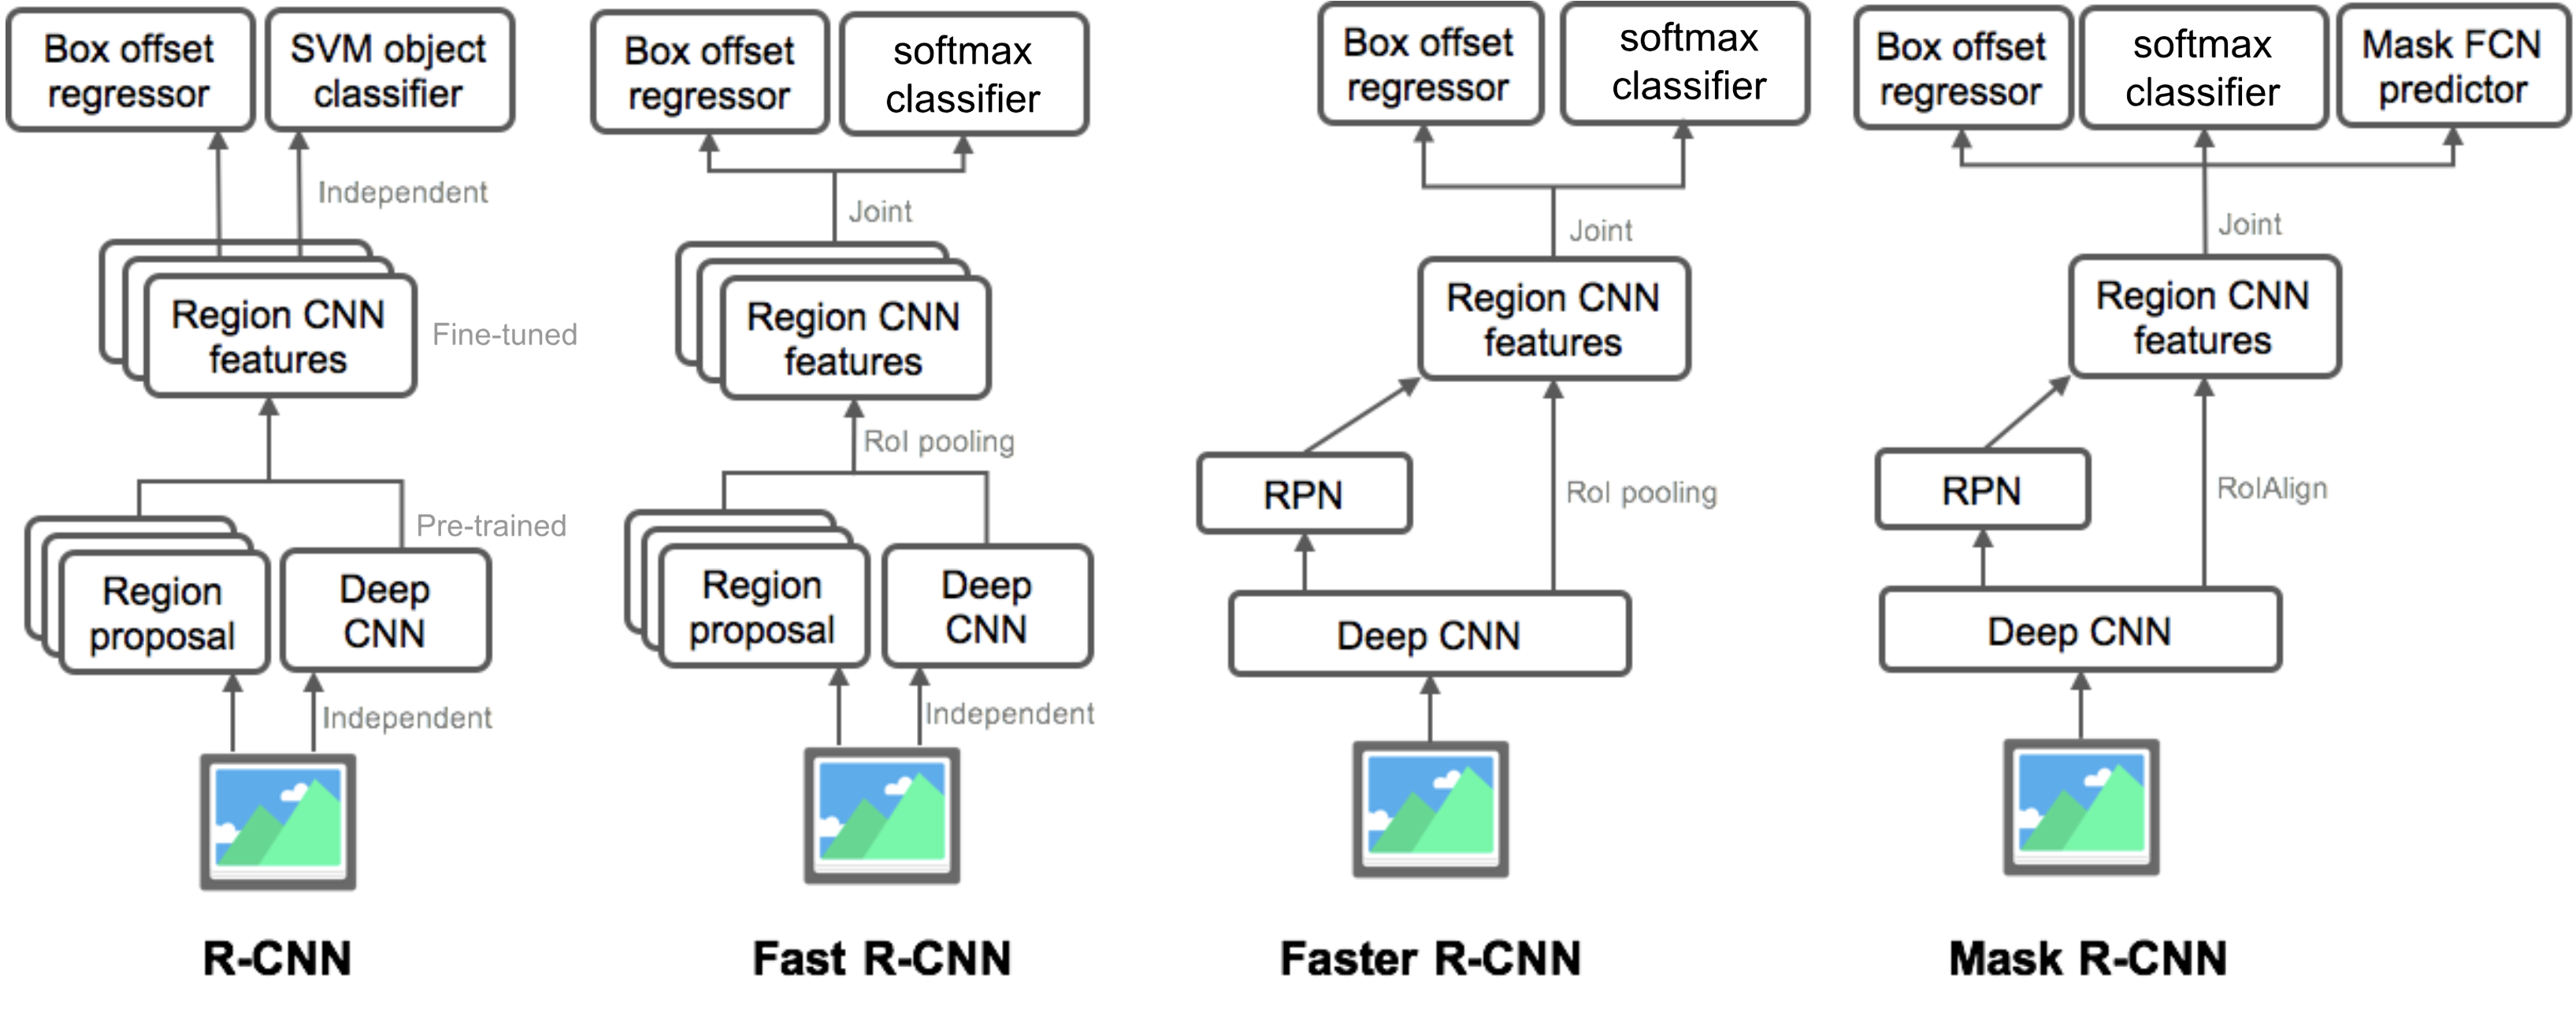
\includegraphics[scale = 0.2]{Sections/2StateOfTheArt/2_images/rcnn-family-summary.png}
        \caption{R-CNN model family summary. \cite{weng2017detection3}} 
    \end{figure}



    \subsection{R-CNN}
    
    \par The principal idea behind Region-based Convolutional Networks (R-CNN) can be split into two steps. In the first step the network identifies a number of regions of interest (bounding-box object region candidate) using a selective search method \cite{weng2017detection3}, which is a common algorithm to provide region proposals that can potentially contain objects \cite{weng2017detection1}.
    \par In the second step it extracts CNN features from each region independently for the classification.

    \begin{figure}[htb]
        \centering
        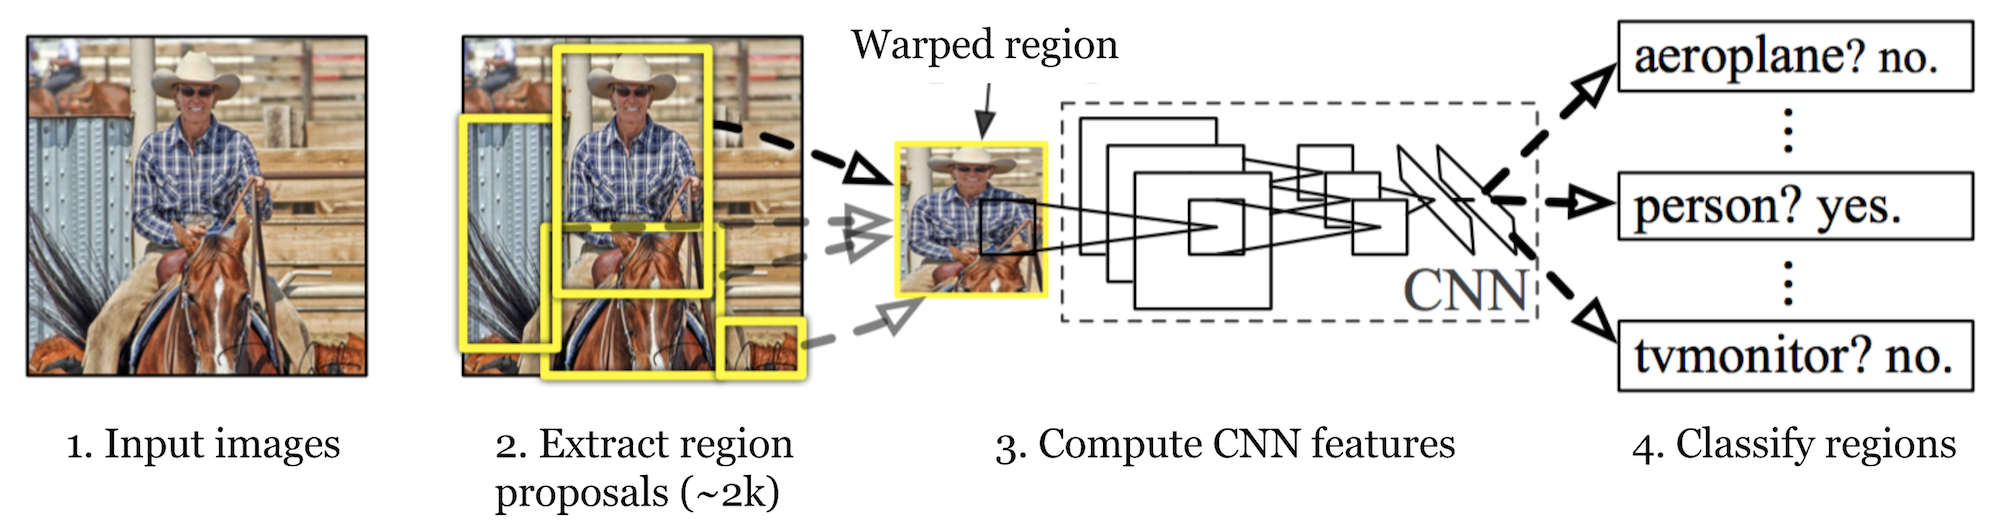
\includegraphics[scale = 0.3]{Sections/2StateOfTheArt/2_images/RCNN.png}
        \caption{R-CNN architecture. \cite{weng2017detection3}} 
    \end{figure}

    \subsection{Fast R-CNN}

    \par The idea behind Fast-RCNN \cite{girshick2015fast} is, as the name implies, to make  R-CNN faster. In order to achieve this, the training procedure was improved by unifying three independent models into one jointly trained framework and increasing shared computation results.
    \par In this new improved network, the CNN feature vectors are not extracted independently for each region proposal, instead this model aggregates them into one CNN forward pass over the entire image and the region proposals share the feature matrix.
    \par This feature matrix is then branched to be used for learning the object classifier and the bounding-box regression.
    \par In short, computation sharing improves the speed of R-CNN. \cite{weng2017detection3}

    \begin{figure}[htb]
        \centering
        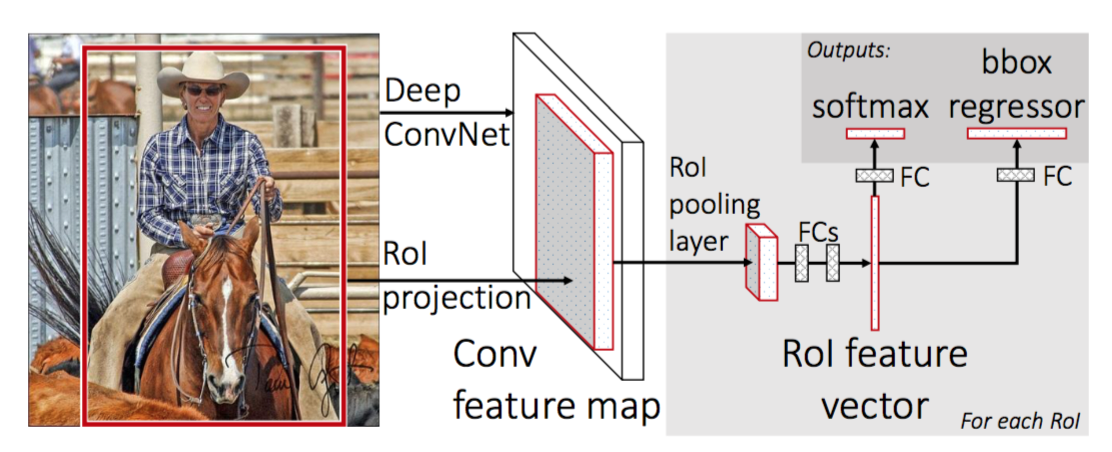
\includegraphics[scale = 0.15]{Sections/2StateOfTheArt/2_images/fast-RCNN.png}
        \caption{Fast R-CNN architecture. \cite{weng2017detection3}} 
    \end{figure}

    
    \subsection{Faster R-CNN}
    \label{sec:fasterrcnn}

    \par The Faster R-CNN \cite{ren2015faster} improves upon the previous considered solutions since it integrates the region proposal algorithm directly into the CNN model. It can be seen as a single, unified model composed of a region proposal network and fast R-CNN with shared convolutional feature layers. \cite{weng2017detection3}

    \begin{figure}[htb]
        \centering
        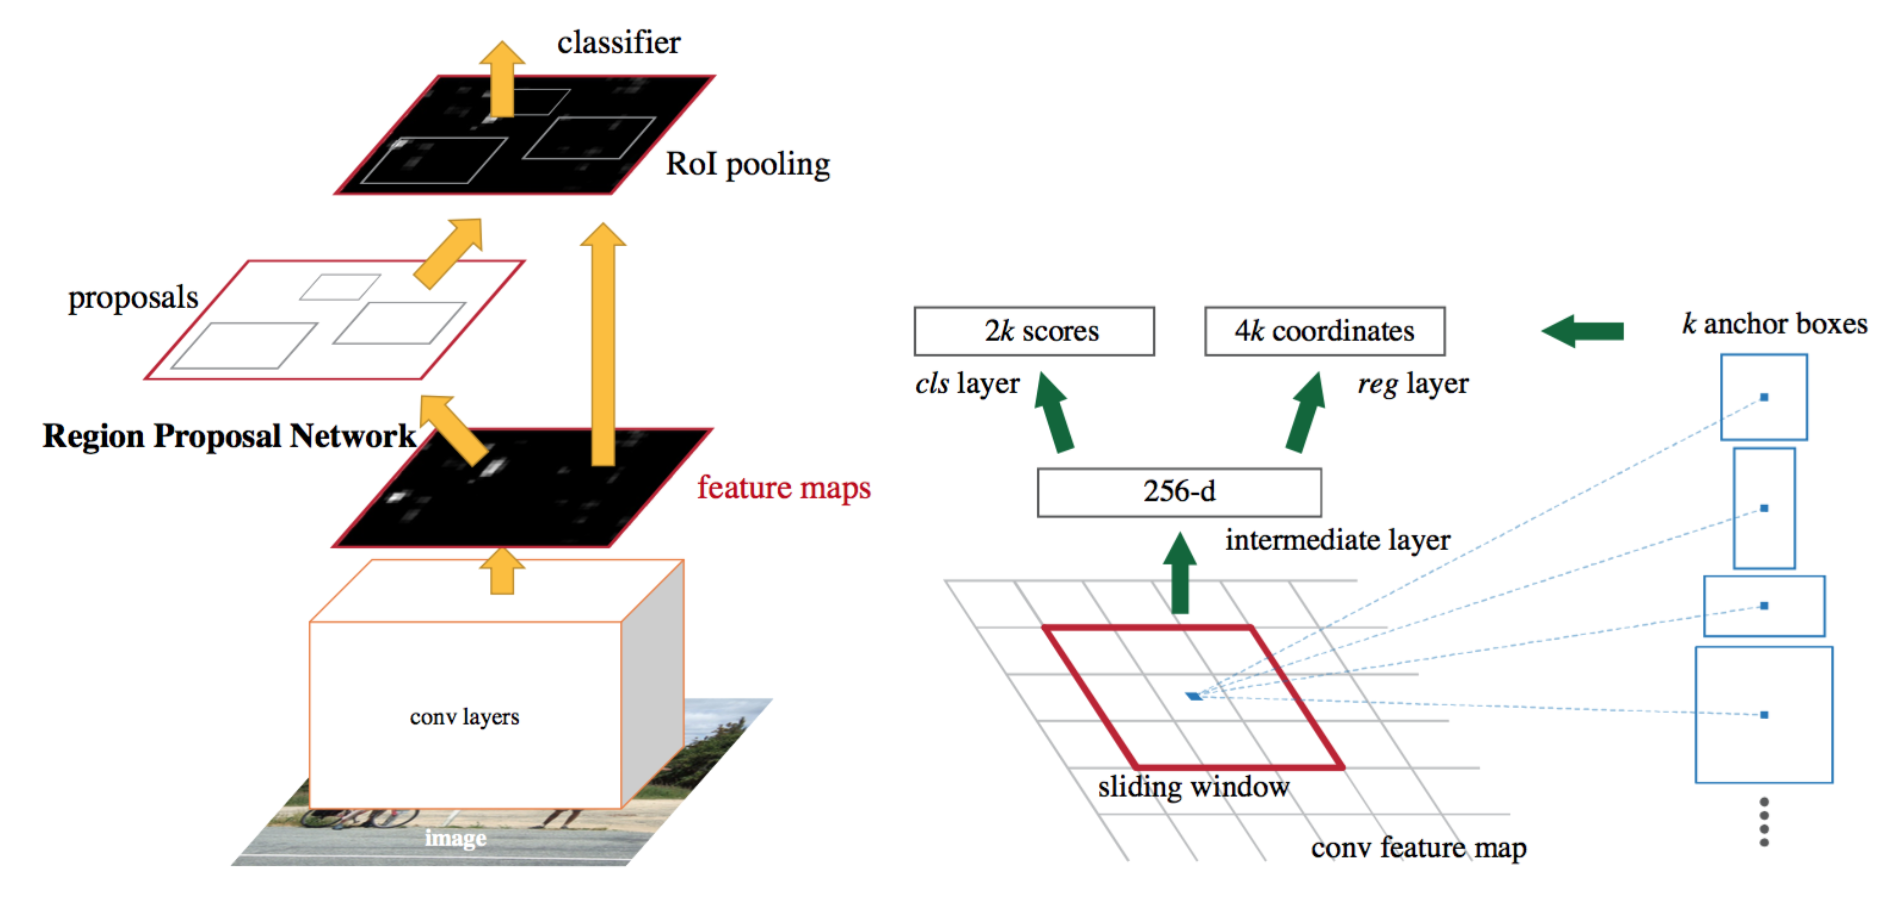
\includegraphics[scale = 0.22]{Sections/2StateOfTheArt/2_images/faster-RCNN.png}
        \caption{Faster R-CNN architecture. \cite{weng2017detection3}} 
    \end{figure}
    

    \subsection{Mask R-CNN}

    \par The final model of the R-CNN family, mask R-CNN \cite{he2017mask}, extends faster R-CNN to pixel-level image segmentation by decoupling the classification and the pixel-level mask prediction tasks. It adds a third branch for predicting an object mask in parallel with existing branches for classification and localization, based of the Faster R-CNN framework.This new mask branch predicts a segmentation mask in a pixel-to-pixel manner.
    \par Mask R-CNN improves the region of interest pooling layer because pixel-level segmentation requires much more fine-grained alignment than bounding boxes. This allows the region of interest to more precisely map regions of the original image. \cite{weng2017detection3}

    \begin{figure}[htb]
        \centering
        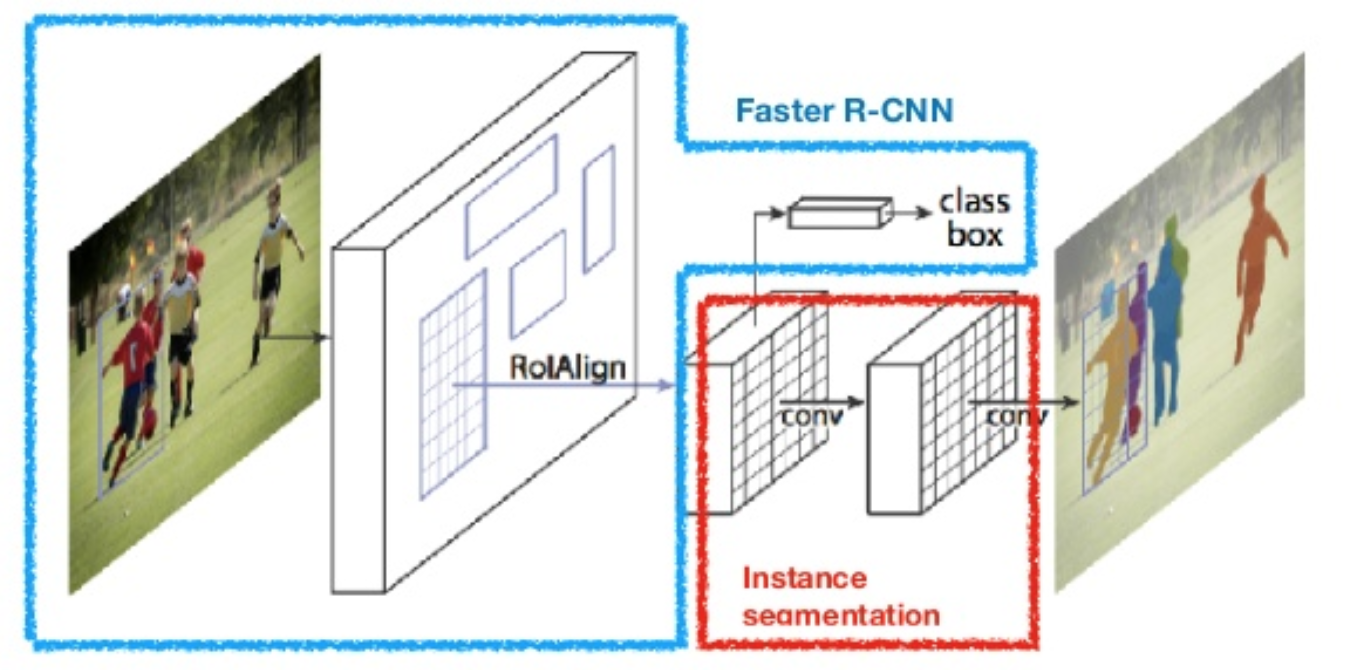
\includegraphics[scale = 0.15]{Sections/2StateOfTheArt/2_images/mask-rcnn.png}
        \caption{Mask R-CNN is a Faster R-CNN model with image segmentation. \cite{weng2017detection3}} 
    \end{figure}

    \newpage  

%%%%%%%%%%%%%%%%%%%%%%%%%%%%%%%%%%%%%%%%%%%%%%%%%%%%%%%%%%%%%%%%%%%%%%%%%%%


\section{State-Of-The-Art}
\label{sec:state}

\par Image classification and object detection are both subjects that are constantly innovating and improving upon previously results, every month new papers are published with new and more efficient networks. 
\par In the figures \ref{fig:leaderboard_object} and \ref{fig:leaderboard_image} it is shown  not only the current best methods for both image classification and object detection but also the development of the state-of-the-art throughout the years.


\begin{figure}[htb]
    \centering
    \includegraphics[scale = 0.25]{Sections/2StateOfTheArt/2_images/chart_object.pdf}
    \caption{Object Detection on COCO test-dev benchmark .\cite{papers_object}} 
    \label{fig:leaderboard_object}
\end{figure}

\begin{figure}[htb]
    \centering
    \includegraphics[scale = 0.25]{Sections/2StateOfTheArt/2_images/chart_image.pdf}
    \caption{Image Classification on ImageNet benchmark. \cite{papers_image}} 
    \label{fig:leaderboard_image}

\end{figure}

\par Due to the fact that object detection is a subject of great innovation, there is an extreme amount of papers that try to compete for the best results coming out every few months. So, in order to do a review of the state of the art the tables, \ref{table:cocotable} and \ref{table:imagenettable} show the benchmarks for both imageNet and COCO test-dev. These tables were obtained from \cite{Ribeiro} and are based on the analysis of \cite{papers_image} and \cite{papers_object} which is a website dedicated to  the current state-of-the-art for object detection and image classification.


\newpage




\subsection{COCO Test-Dev}

\par The COCO benchmark \cite{Lin2014} is a dataset that places object recognition in the context of scene understanding. The evaluation metric used is the average precision (AP). Table \ref{table:cocotable} shows the current best architectures and their respective score for the COCO test-dev dataset.

\begin{table}[htb]
    
    \centering
    \caption {COCO Test-Dev Benchmarks.}
    \begin{tabular}{|| c | c | c | c ||} 
    \hline
    Method & Backbone & AP (\%)  \\ [0.5ex] 
    \hline\hline
    Liu et al.(2019) \cite{Liu2019}  & ResNeXt-152 & 53.3 \\ 
    \hline
    Tan et al. (2019) \cite{Tan2019} & EfficientNet & 51.0 \\
    \hline
    Zhang et al. (2019) \cite{Zhang2019} & ResNeXt-101 & 50.7
    \\
    \hline
    Girshick et al. (2018) \cite{Detectron2018} & ResNeXt-152 & 50.2
    \\
    \hline
    Li et al. (2019) \cite{Li2019} & ResNet-101 & 48.4
    \\ [1ex] 
    \hline
    Zhang et al. (2019) \cite{Zhang2019} & ResNet-101  & 46.3
    \\ [1ex]
    \hline
    Mahajan et al. (2018) \cite{Mahajan2018} & ResNeXt & 45.2
    \\ [1ex]
    \hline
    Zhao et al. (2019) \cite{Zhao2019} & VGG16 & 44.2
    \\ [1ex]
    \hline
    Cai et al. (2018) \cite{Cai2018} & ResNet-101 & 42.8
    \\ [1ex]
    \hline
    Wang et al. (2019) \cite{Wang2019} & ResNet-50    & 39.8
    \\ [1ex]
    \hline
    Lin et al. (2017) \cite{Lin2017} & ResNet-101 & 39.1
    \\ [1ex]
    \hline
    Shrivastava et al. (2016) \cite{shrivastava2016skip} & Inception-ResNet-v2 & 36.8
    \\ [1ex]
    \hline
    Kim et al. (2018) \cite{Kim2018} & VGG-16 & 35.2
    \\ [1ex]
    \hline
   \end{tabular}
   \label{table:cocotable}
\end{table}

\par Liu et al. \cite{Liu2019} achieved the best score in the COCO Test-Dev in 2019. They proposed better detection performance by creating a more powerful backbone network from previously existing backbones like ResNet \cite{He2016} and ResNetXt \cite{Xie2017}. They implemented a strategy for assembling multiple identical backbones (called Assistant Backbones and Lead Backbones) linked by composite connections between the adjacent backbones in order to form a more powerful backbone which was given the name of Composite Backbone Network (CBNet).

\par In typical CNN based detectors, the backbone network (the baseline of a network architecture) is used for basic feature extraction.

\par CBNet feeds the output features of the previous backbone as an input feature to the succeeding backbone through composite connections.At the final stage, the Lead Backbone outputs features for object detection.

\par This architecture was able to achieve the best result in the COCO Test-Dev with a 53.3\% AP with single model by integrating a CBNet using triple ResNeXt-152 \cite{Xie2017} backbones into the Cascade Mask R-CNN baseline.
\par Figure \ref{fig:cbnet} presents the architecture for CBNet.



\begin{figure}[htb]
    \centering
    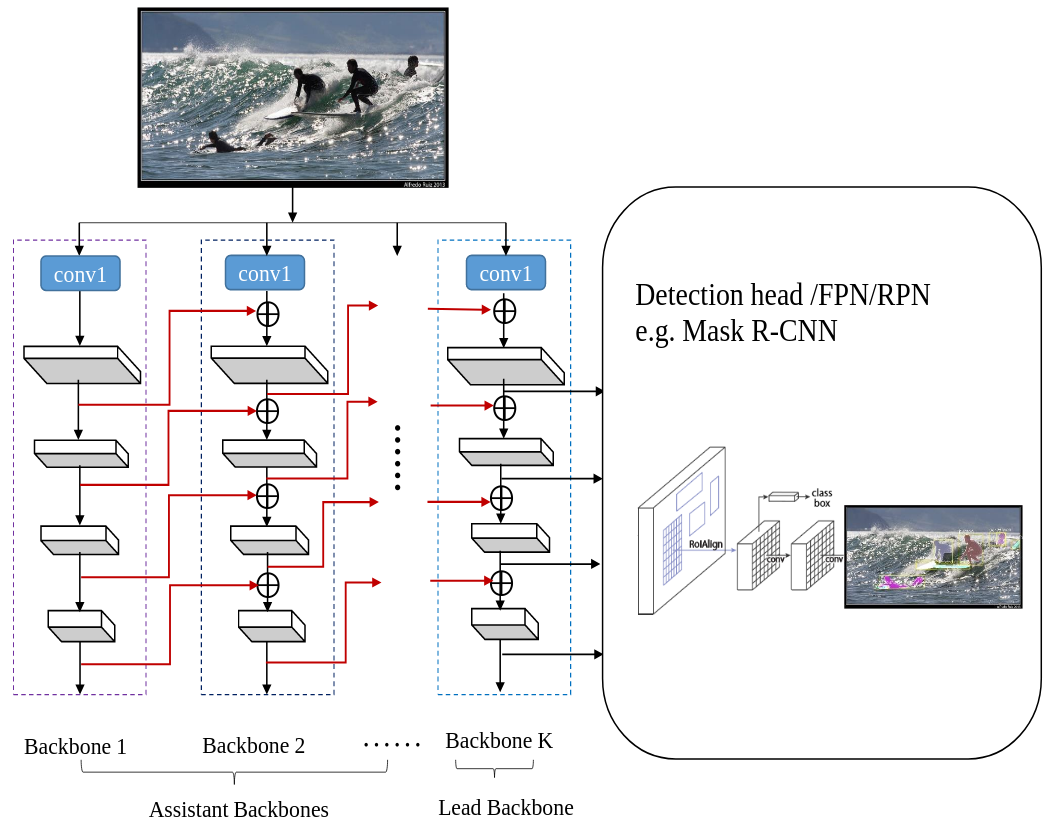
\includegraphics[scale = 0.25]{Sections/2StateOfTheArt/2_images/cbnet.png}
    \caption{CBNet Architecture for object detection.} 
    \label{fig:cbnet}
\end{figure}

\subsubsection{ResNeXt}
\label{sec:resnext}
\par ResNeXt, also known as Aggregated Residual Transform Network was created by facebook researchers and it is a simple highly modularized network architecture for image classification. 
\par The network is constructed by repeating a building block that aggregates a set of transformations with the same topology. The simple design results in a homogeneous, multi-branch architecture that has only a few hyper-parameters to set. This strategy creates a new dimension, which was given the name of "cardinality" (size of the set of transformations). 
\par This architecture is an improvement over the Inception architectures, being more simple in design and adding more branches (towers) within modules. \cite{Xie2017}


\begin{figure}[htb]
    \centering
    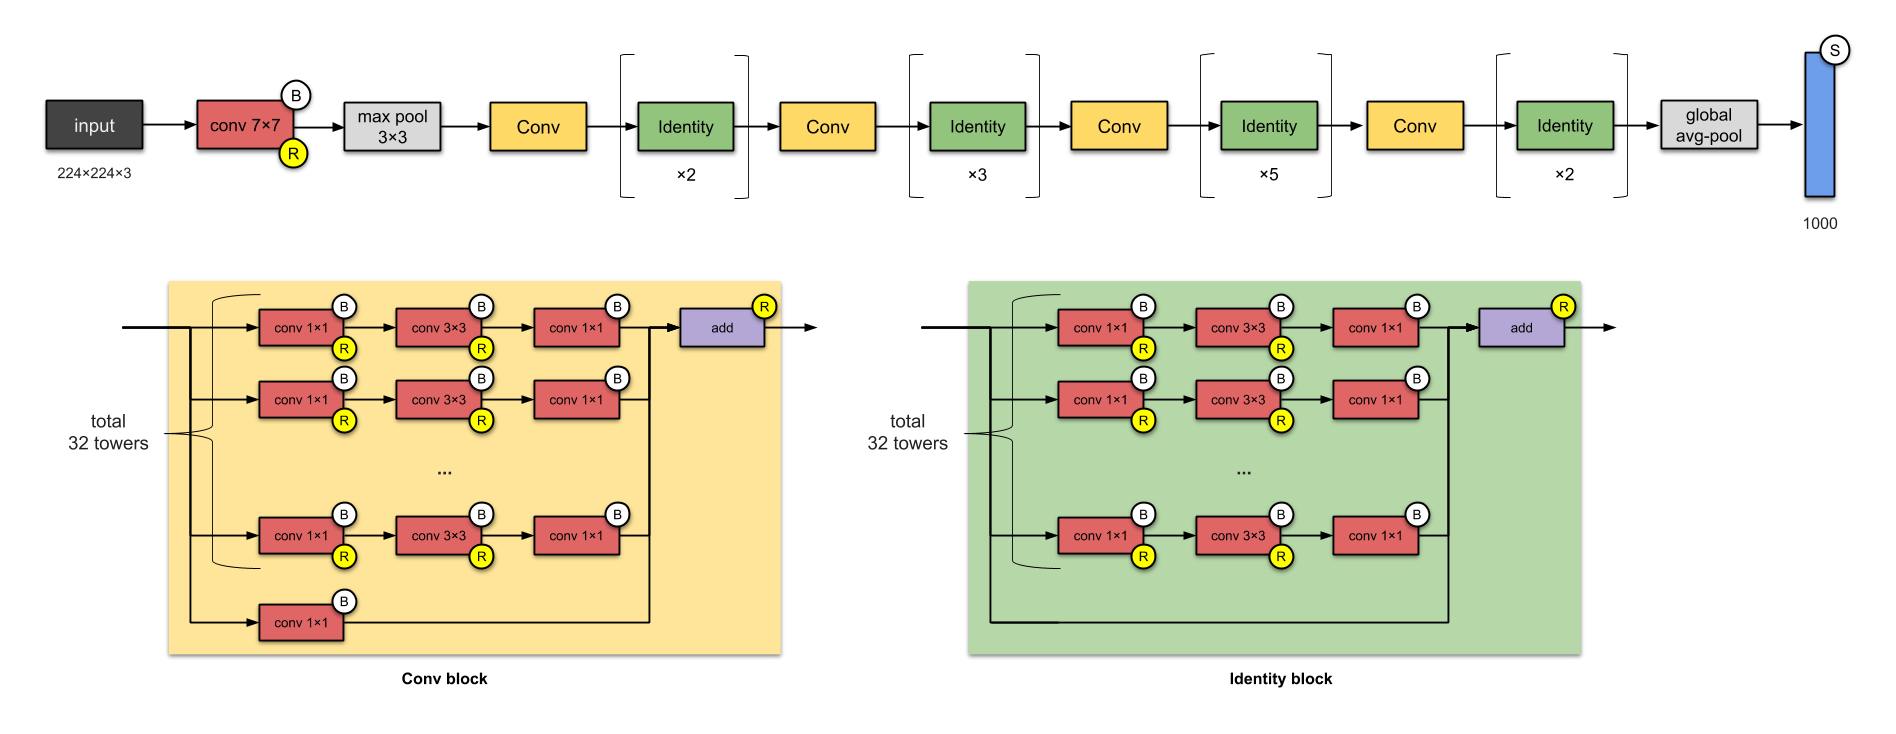
\includegraphics[scale = 0.23]{Sections/2StateOfTheArt/2_images/resnext.png}
    \caption{ResNeXt architecture. \cite{cnnarchitectures} }
    \label{fig:noisestudent}
\end{figure}


\newpage

\subsection{ImageNet}
\par The imageNet Large Scale Visual Recognition challenge \cite{Russakovsky2015} is a benchmark for object category classification and detection. The evaluation metrics used are top-1 and top-5 accuracy.

\begin{table}[htb]
    
    \centering
    \caption {ImageNet Benchmarks.}
    \begin{tabular}{|| c | c | c ||} 
    \hline
    Method & Backbone & Top-1 Acc (\%)  \\ [0.5ex] 
    \hline\hline
    Xie et al. (2019) \cite{Xie2019}& EfficientNet & 88.4
    \\ 
    \hline
    Kolesnikov et al. (2019) \cite{alex2019large} & ResNet-152 & 87.8

    \\
    \hline
    Touvron et al. (2019) \cite{touvron2019fixing} & ResNeXt-101 & 86.4

    \\
    \hline
    Xie et al. (2019) \cite{xie2019adversarial} & EfficientNet & 85.5

    \\ [1ex] 
    \hline
    Mahajan et al. (2018) \cite{Mahajan2018} & ResNeXt & 85.4

    \\ [1ex]
    \hline
    Tan et al. (2019) \cite{tan2019efficientnet}& EfficientNet & 84.4

    \\ [1ex]
    \hline
    Touvron et al. (2019) \cite{touvron2019fixing} & ResNet-50 & 82.5

    \\ [1ex]
    \hline
    Szegedy et al. (2017) \cite{szegedy2016inceptionv4} & Inception-resnet-v2 & 80.1

    \\ [1ex]
    \hline
    Szegedy et al. (2017) \cite{szegedy2016inceptionv4}  & Inception-v4 & 80.0

    \\ [1ex]
    \hline
    Simonyan et al. (2014) \cite{simonyan2014deep} & VGG-16 & 74.4
    \\ [1ex]
    \hline
   \end{tabular}
   \label{table:imagenettable}
\end{table}



\par Xie et al. \cite{Xie2019} stated that current state-of-the-art vision models are still trained with supervised learning, which implies the necessity of large corpus of labeled images in order to work properly. The fact that current models are only shown labeled images causes an obvious limitations in the improvement of accuracy and robustness of current state-of-the-art models, this can be improved with the usage of the large available quantities of unlabeled images available.
\par Having this in mind, they decided to use unlabeled images to improve the state-of-the-art ImageNet accuracy and show that accuracy has an outsized impact on robustness. For this purpose, they used a much larger corpus of unlabeled images, where a large fraction of images did not belong to ImageNet training set distribution.
\par Using a self-training framework the model was trained with 3 main steps which consist in:

\begin{enumerate}
    \item Training of a teacher model on labeled images.
    \item Usage of the teacher to generate pseudo labels on unlabeled images.
    \item Train a student model on the combination of labeled images.
\end{enumerate}

\par The algorithm was iterated a few times by treating the student as a teacher to relabel the unlabeled data and training a new student.

\par An important discovery was made during the training of the algorithm. For the method to work well at scale the student model should be noised during its training while the teacher should not be noised during the generation of pseudo labels. This way, the pseudo labels are as accurate as possible and the noised student is forced to learn harder from the pseudo labels. To induce noise in the model it was used RandAugment data, dropout and stochastic depth during the training. Figure \ref{fig:noisestudent} shows a brief view of how the method works.
\par This is where the name of the method "Noisy Student"comes from, since the student is noised to learn beyond the teacher's knowledge.
\par With this method they were able to show that it is possible to use unlabeled images to significantly advance both accuracy and robustness of state-of-the-art imageNet models.
\par The presented model uses EfficientNet (this architecture is explained in more detail in \ref{sec:efficientNet}) as a backbone trained on images from imageNet dataset and was able to obtain the best results in the ImageNet benchmark dataset by achieving an accuracy of 88.4\%.



\begin{figure}[htb]
    \centering
    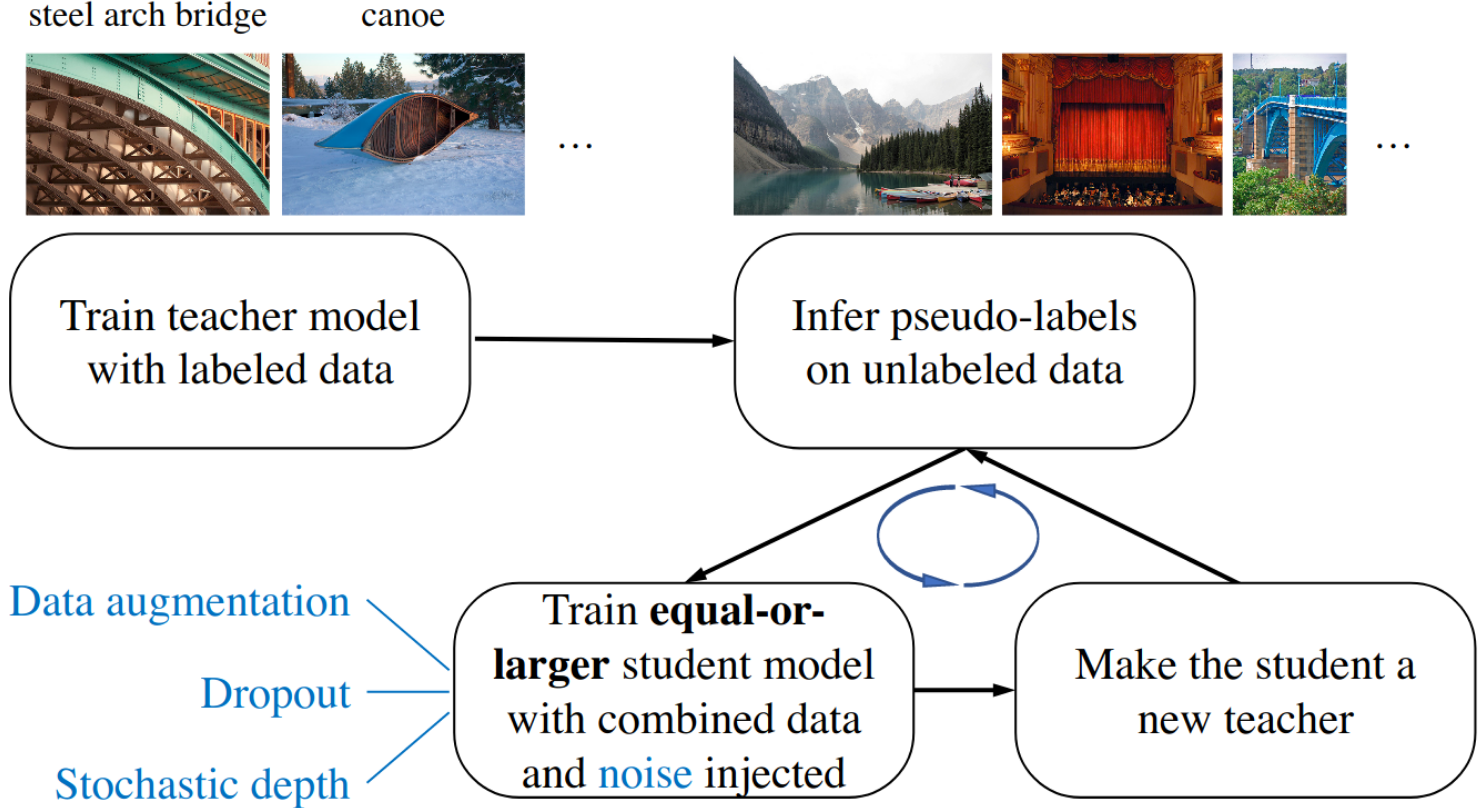
\includegraphics[scale = 0.15]{Sections/2StateOfTheArt/2_images/noisy_student.png}
    \caption{Noisy Student Method. \cite{Xie2019}} 
    \label{fig:noisestudent}
\end{figure}cnnarchitectures

\par Researchers at Google decided to study the impact of scaling up CNNs, in order to achieve better accuracy and efficiency. EfficientNet-B0 was developed based on a simple idea, scaling each of the dimensions of the network (width, depth and resolution) with a constant ratio, improves the overall performance \cite{tan2019efficientnet}.

\begin{figure}[htb]
    \centering
    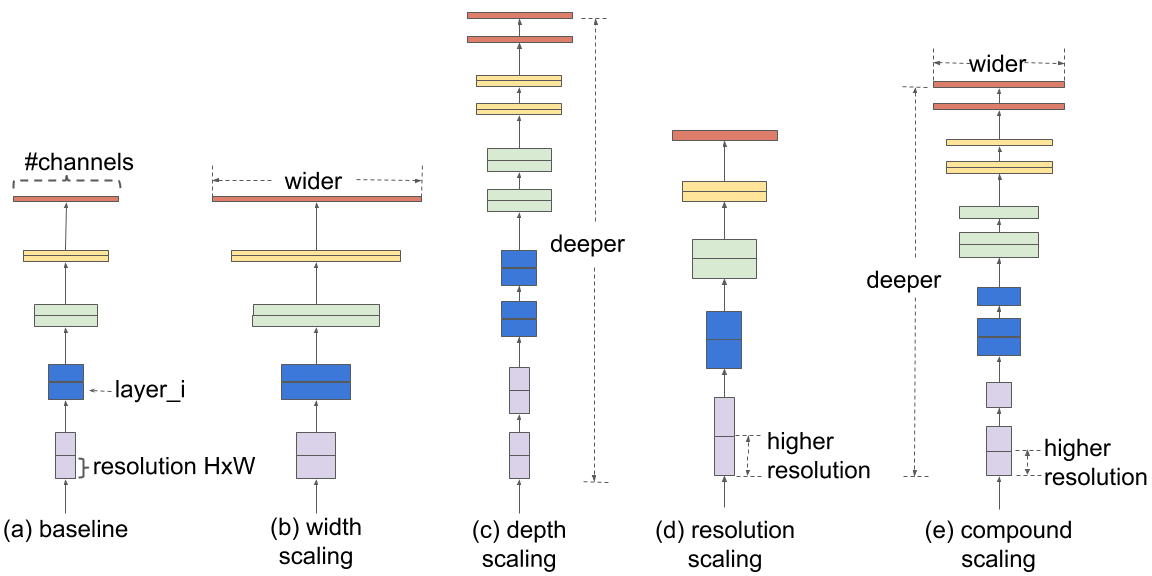
\includegraphics[scale = 0.25]{Sections/2StateOfTheArt/2_images/efficientNet_scale.png}
    \caption{Comparison of different scaling methods:  (a) is a baseline network example; (b)-(d) are conventional scaling that only increases one dimension of network  width, depth, or resolution. (e) is the proposed compound scaling method that uniformly scales all three dimensions with a fixed ratio. \cite{tan2019efficientnet}
    } 

\end{figure}

\newpage

\par The baseline network architecture, EffecientNet-B0, uses mobile inverted bottleneck convolution (MBConv), similar to MobileNetV2 \cite{s2018mobilenetv2} and MnasNet \cite{tan2018mnasnet}. Figure  shows the baseline network architecture EfficientNet-B0.

\begin{figure}[htb]
    \centering
    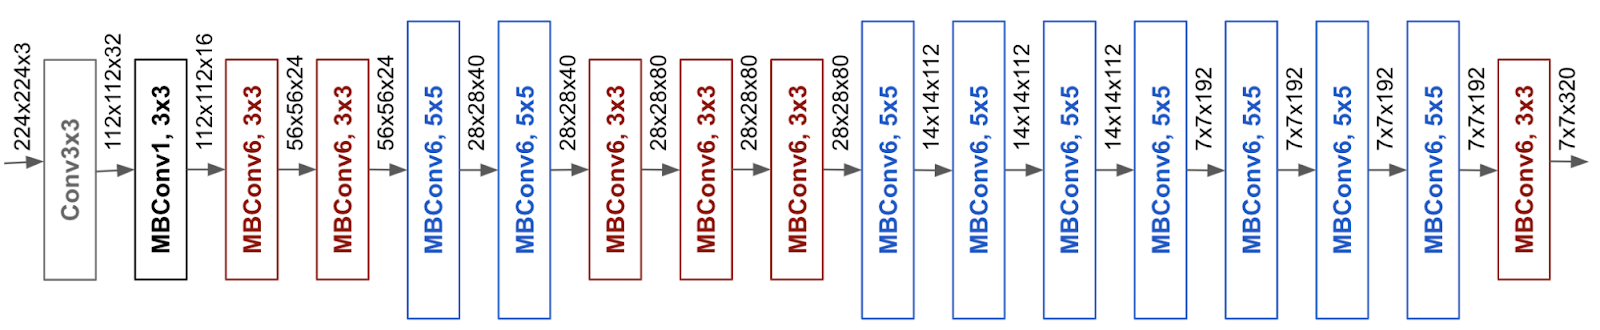
\includegraphics[scale = 0.22]{Sections/2StateOfTheArt/2_images/efficientNet_Arch.png}
    \caption{EfficientNet-B0 architecture representation.} 

\end{figure}